\nonstopmode
\documentclass[12pt]{report} 
\usepackage{hyperref}
\usepackage{bookmark}
\hypersetup{colorlinks=true,linkcolor=blue}
\usepackage{theorem,graphicx}
\usepackage{listings,alltt}
\usepackage[final]{pdfpages}
\bibliographystyle{plain}
\usepackage{tocloft}



\lstset{ %configuring the display of scilab codes
             tabsize=4,
             language=scilab,
             basicstyle=\ttfamily,
             aboveskip={1\baselineskip},
             showstringspaces=false,
             breaklines=true,
             showspaces=false,
             numbers=left,
             numberstyle=\small,
             stringstyle=\normalfont,
             keywordstyle=\color{red},
             emph={clc, all, gca},
             emphstyle=\color{red},
             commentstyle=\color{blue}\normalfont}

 
% code environment
{\theorembodyfont{\rmfamily} \newtheorem{codemass}{Scilab code}[chapter]}
\newenvironment{code}%
{\begin{codemass}}{\hrule \end{codemass}}

{\theorembodyfont{\rmfamily} \newtheorem{accmass}{Acc}[chapter]}
\newenvironment{acc-code}%
{\begin{accmass}}{\end{accmass}}


% create listing for code

\newcommand\tcaption[1]
     {\addcontentsline{cod}{section}{\protect\numberline {\thecodemass}#1}}
\makeatletter \newcommand\listofcode
     {\chapter*{List of Scilab Codes\markboth%
                        {\bf List of Scilab Codes}{}}%
\renewcommand*\l@section{\@dottedtocline{1}{5em}{6em}}%
\addcontentsline{toc}{chapter}{\protect\numberline{List of Scilab Codes}}
\@starttoc{cod}}
\newcommand\l@matlab[3]
     {#1 \par\noindent#2, #3 \par}
\renewcommand\@pnumwidth{2.1em}
%\makeatother

\makeatletter
\def\curlable#1{\def\thecodemass{#1}\def\@currentlabel{#1}}
\makeatother

\newcommand{\coderef}[1]{Exa~\ref{#1}}
\newcommand{\figref}[1]{Fig.~\ref{#1}}

\title{Scilab Textbook Companion for \\Fundamental Of Physics\\by D. Haliday, R. Resnick And J. Walker\footnote{Funded by a grant from the National Mission on Education through ICT, http://spoken-tutorial.org/NMEICT-Intro. This Textbook Companion and Scilab codes written in it can be downloaded from the "Textbook Companion Project" section at the website http://scilab.in}}
\author{ Created by \\Aman Mangal\\B.TECH (pursuing)\\Computer Engineering\\IIT Bombay\\ College Teacher\\Not Decided\\Cross-Checked by \\Prashant Dave, IIT Bombay\\}
\date{\today}
\begin{document}
\maketitle

\chapter*{Book Description}
\begin{description}
\item [Title:] Fundamental Of Physics
\item [Author:] D. Haliday, R. Resnick And J. Walker
\item [Publisher:] John Wiley And Sons Inc.
\item [Edition:] 6
\item [Year:] 2011
\item [ISBN:] 9971-51-330-7
\end{description}

\newpage
\vspace*{3cm}
Scilab numbering policy used in this document and the relation to the above book.
\begin{description}
\item[Exa] Example (Solved example)
\item[Eqn] Equation (Particular equation of the above book)
\item[AP] Appendix to Example(Scilab Code that is an Appednix to a particular Example of the above book)
\end{description}
For example, Exa~3.51 means solved example 3.51 of this book. Sec~2.3 means a scilab code whose theory is explained in Section 2.3 of the book.

\newpage
\vspace*{3cm}
\tableofcontents
\listofcode
\newpage
\vspace*{3cm}
\listoffigures
\chapter{Measurement}

\vspace*{10mm}
\curlable{Exa~1.1}
\begin{code}
\tcaption{Sample Problem 1}
\begin{verbatim}
Sample Problem 1
\end{verbatim}
\lstinputlisting{../24/CH1/EX1.1/Example1_1.sce}
\end{code}

\vspace*{10mm}
\vspace*{10mm}
\curlable{Exa~1.2}
\begin{code}
\tcaption{Sample Problem 2}
\begin{verbatim}
Sample Problem 2
\end{verbatim}
\lstinputlisting{../24/CH1/EX1.2/Example1_2.sce}
\end{code}

\vspace*{10mm}
\vspace*{10mm}
\curlable{Exa~1.3}
\begin{code}
\tcaption{Sample Problem 3}
\begin{verbatim}
Sample Problem 3
\end{verbatim}
\lstinputlisting{../24/CH1/EX1.3/Example1_3.sce}
\end{code}

\vspace*{10mm}
\vspace*{10mm}
\curlable{Exa~1.4}
\begin{code}
\tcaption{Sample Problem 4}
\begin{verbatim}
Sample Problem 4
\end{verbatim}
\lstinputlisting{../24/CH1/EX1.4/Example1_4.sce}
\end{code}

\vspace*{10mm}
\chapter{Motion Along a Straight Line}

\vspace*{10mm}
\curlable{Exa~2.1.a}
\begin{code}
\tcaption{Sample Problem 1a}
\begin{verbatim}
Sample Problem 1a
\end{verbatim}
\lstinputlisting{../24/CH2/EX2.1.a/Example2_1a.sce}
\end{code}

\vspace*{10mm}
check Appendix \ref{AP:275} for dependency: {\begin{alltt} \hspace{2mm} Example2_1a.sce \end{alltt}}

\vspace*{10mm}
\curlable{Exa~2.1.b}
\begin{code}
\tcaption{Sample Problem 1b}
\begin{verbatim}
Sample Problem 1b
\end{verbatim}
\lstinputlisting{../24/CH2/EX2.1.b/Example2_1b.sce}
\end{code}

\vspace*{10mm}
check Appendix \ref{AP:275} for dependency: {\begin{alltt} \hspace{2mm} Example2_1a.sce \end{alltt}}

check Appendix \ref{AP:276} for dependency: {\begin{alltt} \hspace{2mm} Example2_1b.sce \end{alltt}}

\vspace*{10mm}
\curlable{Exa~2.1.c}
\begin{code}
\tcaption{Sample Problem 1c}
\begin{verbatim}
Sample Problem 1c
\end{verbatim}
\lstinputlisting{../24/CH2/EX2.1.c/Example2_1c.sce}
\end{code}

\vspace*{10mm}
\curlable{Fig~2.1.c}
\begin{figure}
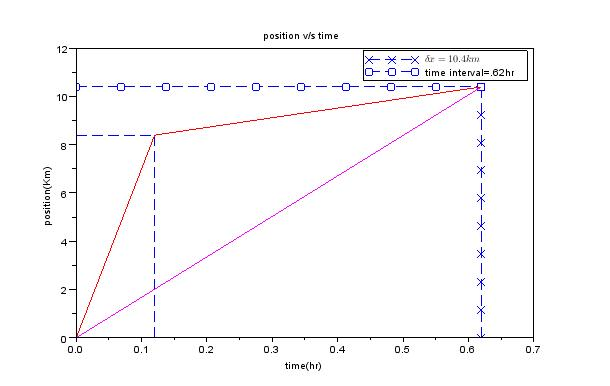
\includegraphics[width=5in]{../24/CH2/EX2.1.c/Example2_1c_graph.jpg}
\caption{Sample Problem 1c}
\end{figure}

\vspace*{10mm}
check Appendix \ref{AP:275} for dependency: {\begin{alltt} \hspace{2mm} Example2_1a.sce \end{alltt}}

check Appendix \ref{AP:276} for dependency: {\begin{alltt} \hspace{2mm} Example2_1b.sce \end{alltt}}

\vspace*{10mm}
\curlable{Exa~2.1.d}
\begin{code}
\tcaption{Sample Problem 1d}
\begin{verbatim}
Sample Problem 1d
\end{verbatim}
\lstinputlisting{../24/CH2/EX2.1.d/Example2_1d.sce}
\end{code}

\vspace*{10mm}
\vspace*{10mm}
\curlable{Exa~2.2}
\begin{code}
\tcaption{Sample Problem 2}
\begin{verbatim}
Sample Problem 2
\end{verbatim}
\lstinputlisting{../24/CH2/EX2.2/Example2_2.sce}
\end{code}

\vspace*{10mm}
\curlable{Fig~2.2}
\begin{figure}
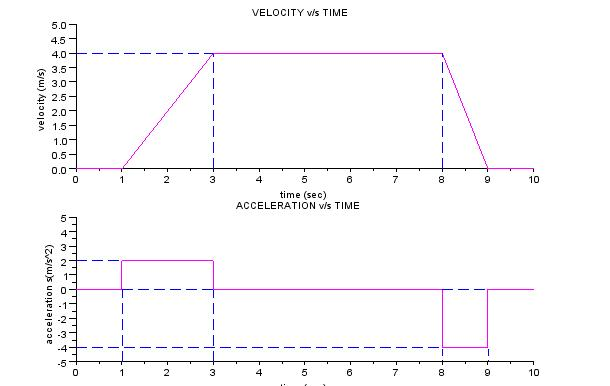
\includegraphics[width=5in]{../24/CH2/EX2.2/Example2_2_graph.jpg}
\caption{Sample Problem 2}
\end{figure}

\vspace*{10mm}
\vspace*{10mm}
\curlable{Exa~2.3}
\begin{code}
\tcaption{Sample Problem 3}
\begin{verbatim}
Sample Problem 3
\end{verbatim}
\lstinputlisting{../24/CH2/EX2.3/Example2_3.sce}
\end{code}

\vspace*{10mm}
\vspace*{10mm}
\curlable{Exa~2.4}
\begin{code}
\tcaption{Sample Problem 4}
\begin{verbatim}
Sample Problem 4
\end{verbatim}
\lstinputlisting{../24/CH2/EX2.4/Example2_4.sce}
\end{code}

\vspace*{10mm}
\vspace*{10mm}
\curlable{Exa~2.5}
\begin{code}
\tcaption{Sample Problem 5}
\begin{verbatim}
Sample Problem 5
\end{verbatim}
\lstinputlisting{../24/CH2/EX2.5/Example2_5.sce}
\end{code}

\vspace*{10mm}
\vspace*{10mm}
\curlable{Exa~2.6}
\begin{code}
\tcaption{Sample Problem 6}
\begin{verbatim}
Sample Problem 6
\end{verbatim}
\lstinputlisting{../24/CH2/EX2.6/Example2_6.sce}
\end{code}

\vspace*{10mm}
\vspace*{10mm}
\curlable{Exa~2.7}
\begin{code}
\tcaption{Sample Problem 7}
\begin{verbatim}
Sample Problem 7
\end{verbatim}
\lstinputlisting{../24/CH2/EX2.7/Example2_7.sce}
\end{code}

\vspace*{10mm}
\chapter{Vectors}

check Appendix \ref{AP:272} for dependency: {\begin{alltt} \hspace{2mm} degree_rad.sci \end{alltt}}

\vspace*{10mm}
\curlable{Exa~3.1}
\begin{code}
\tcaption{Sample Problem 1}
\begin{verbatim}
Sample Problem 1
\end{verbatim}
\lstinputlisting{../24/CH3/EX3.1/Example3_1.sce}
\end{code}

\vspace*{10mm}
check Appendix \ref{AP:272} for dependency: {\begin{alltt} \hspace{2mm} degree_rad.sci \end{alltt}}

\vspace*{10mm}
\curlable{Exa~3.2}
\begin{code}
\tcaption{Sample Problem 2}
\begin{verbatim}
Sample Problem 2
\end{verbatim}
\lstinputlisting{../24/CH3/EX3.2/Example3_2.sce}
\end{code}

\vspace*{10mm}
check Appendix \ref{AP:272} for dependency: {\begin{alltt} \hspace{2mm} degree_rad.sci \end{alltt}}

\vspace*{10mm}
\curlable{Exa~3.3}
\begin{code}
\tcaption{Sample Problem 3}
\begin{verbatim}
Sample Problem 3
\end{verbatim}
\lstinputlisting{../24/CH3/EX3.3/Example3_3.sce}
\end{code}

\vspace*{10mm}
check Appendix \ref{AP:272} for dependency: {\begin{alltt} \hspace{2mm} degree_rad.sci \end{alltt}}

\vspace*{10mm}
\curlable{Exa~3.4}
\begin{code}
\tcaption{Sample Problem 4}
\begin{verbatim}
Sample Problem 4
\end{verbatim}
\lstinputlisting{../24/CH3/EX3.4/Example3_4.sce}
\end{code}

\vspace*{10mm}
check Appendix \ref{AP:272} for dependency: {\begin{alltt} \hspace{2mm} degree_rad.sci \end{alltt}}

\vspace*{10mm}
\curlable{Exa~3.5}
\begin{code}
\tcaption{Sample Problem 5}
\begin{verbatim}
Sample Problem 5
\end{verbatim}
\lstinputlisting{../24/CH3/EX3.5/Example3_5.sce}
\end{code}

\vspace*{10mm}
check Appendix \ref{AP:272} for dependency: {\begin{alltt} \hspace{2mm} degree_rad.sci \end{alltt}}

\vspace*{10mm}
\curlable{Exa~3.6}
\begin{code}
\tcaption{Sample Problem 6}
\begin{verbatim}
Sample Problem 6
\end{verbatim}
\lstinputlisting{../24/CH3/EX3.6/Example3_6.sce}
\end{code}

\vspace*{10mm}
check Appendix \ref{AP:277} for dependency: {\begin{alltt} \hspace{2mm} cross_product.sci \end{alltt}}

check Appendix \ref{AP:272} for dependency: {\begin{alltt} \hspace{2mm} degree_rad.sci \end{alltt}}

\vspace*{10mm}
\curlable{Exa~3.7}
\begin{code}
\tcaption{Sample Problem 7}
\begin{verbatim}
Sample Problem 7
\end{verbatim}
\lstinputlisting{../24/CH3/EX3.7/Example3_7.sce}
\end{code}

\vspace*{10mm}
check Appendix \ref{AP:277} for dependency: {\begin{alltt} \hspace{2mm} cross_product.sci \end{alltt}}

check Appendix \ref{AP:272} for dependency: {\begin{alltt} \hspace{2mm} degree_rad.sci \end{alltt}}

\vspace*{10mm}
\curlable{Exa~3.8}
\begin{code}
\tcaption{Sample Problem 8}
\begin{verbatim}
Sample Problem 8
\end{verbatim}
\lstinputlisting{../24/CH3/EX3.8/Example3_8.sce}
\end{code}

\vspace*{10mm}
\chapter{Motion in Two and Three Dimesions}

\vspace*{10mm}
\curlable{Exa~4.1}
\begin{code}
\tcaption{Sample Problem 1}
\begin{verbatim}
Sample Problem 1
\end{verbatim}
\lstinputlisting{../24/CH4/EX4.1/Example4_1.sce}
\end{code}

\vspace*{10mm}
\vspace*{10mm}
\curlable{Exa~4.2.a}
\begin{code}
\tcaption{Sample Problem 2a}
\begin{verbatim}
Sample Problem 2a
\end{verbatim}
\lstinputlisting{../24/CH4/EX4.2.a/Example4_2a.sce}
\end{code}

\vspace*{10mm}
check Appendix \ref{AP:272} for dependency: {\begin{alltt} \hspace{2mm} degree_rad.sci \end{alltt}}

check Appendix \ref{AP:278} for dependency: {\begin{alltt} \hspace{2mm} Example4_2a.sce \end{alltt}}

\vspace*{10mm}
\curlable{Exa~4.2.b}
\begin{code}
\tcaption{Sample Problem 2b}
\begin{verbatim}
Sample Problem 2b
\end{verbatim}
\lstinputlisting{../24/CH4/EX4.2.b/Example4_2b.sce}
\end{code}

\vspace*{10mm}
\curlable{Fig~4.2.b}
\begin{figure}
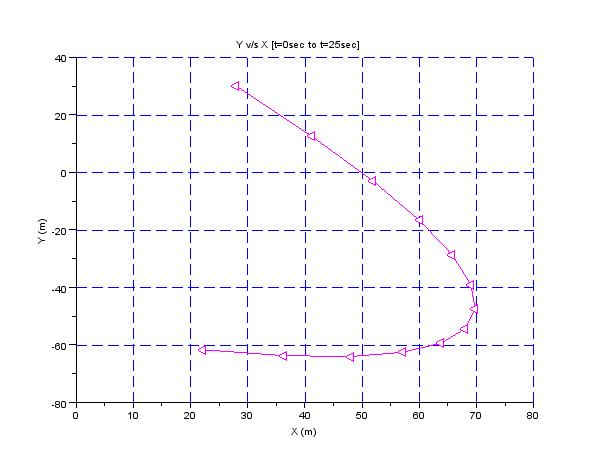
\includegraphics[width=5in]{../24/CH4/EX4.2.b/Example4_2b_graph.jpg}
\caption{Sample Problem 2b}
\end{figure}

\vspace*{10mm}
check Appendix \ref{AP:278} for dependency: {\begin{alltt} \hspace{2mm} Example4_2a.sce \end{alltt}}

\vspace*{10mm}
\curlable{Exa~4.3}
\begin{code}
\tcaption{Sample Problem 3}
\begin{verbatim}
Sample Problem 3
\end{verbatim}
\lstinputlisting{../24/CH4/EX4.3/Example4_3.sce}
\end{code}

\vspace*{10mm}
check Appendix \ref{AP:279} for dependency: {\begin{alltt} \hspace{2mm} Example4_3.sce \end{alltt}}

\vspace*{10mm}
\curlable{Exa~4.4}
\begin{code}
\tcaption{Sample Problem 4}
\begin{verbatim}
Sample Problem 4
\end{verbatim}
\lstinputlisting{../24/CH4/EX4.4/Example4_4.sce}
\end{code}

\vspace*{10mm}
check Appendix \ref{AP:272} for dependency: {\begin{alltt} \hspace{2mm} degree_rad.sci \end{alltt}}

\vspace*{10mm}
\curlable{Exa~4.5}
\begin{code}
\tcaption{Sample Problem 5}
\begin{verbatim}
Sample Problem 5
\end{verbatim}
\lstinputlisting{../24/CH4/EX4.5/Example4_5.sce}
\end{code}

\vspace*{10mm}
check Appendix \ref{AP:272} for dependency: {\begin{alltt} \hspace{2mm} degree_rad.sci \end{alltt}}

\vspace*{10mm}
\curlable{Exa~4.6}
\begin{code}
\tcaption{Sample Problem 6}
\begin{verbatim}
Sample Problem 6
\end{verbatim}
\lstinputlisting{../24/CH4/EX4.6/Example4_6.sce}
\end{code}

\vspace*{10mm}
check Appendix \ref{AP:272} for dependency: {\begin{alltt} \hspace{2mm} degree_rad.sci \end{alltt}}

\vspace*{10mm}
\curlable{Exa~4.7}
\begin{code}
\tcaption{Sample Problem 7}
\begin{verbatim}
Sample Problem 7
\end{verbatim}
\lstinputlisting{../24/CH4/EX4.7/Example4_7.sce}
\end{code}

\vspace*{10mm}
check Appendix \ref{AP:272} for dependency: {\begin{alltt} \hspace{2mm} degree_rad.sci \end{alltt}}

\vspace*{10mm}
\curlable{Exa~4.8}
\begin{code}
\tcaption{Sample Problem 8}
\begin{verbatim}
Sample Problem 8
\end{verbatim}
\lstinputlisting{../24/CH4/EX4.8/Example4_8.sce}
\end{code}

\vspace*{10mm}
\vspace*{10mm}
\curlable{Exa~4.9}
\begin{code}
\tcaption{Sample Problem 9}
\begin{verbatim}
Sample Problem 9
\end{verbatim}
\lstinputlisting{../24/CH4/EX4.9/Example4_9.sce}
\end{code}

\vspace*{10mm}
\vspace*{10mm}
\curlable{Exa~4.10}
\begin{code}
\tcaption{Sample Problem 10}
\begin{verbatim}
Sample Problem 10
\end{verbatim}
\lstinputlisting{../24/CH4/EX4.10/Example4_10.sce}
\end{code}

\vspace*{10mm}
check Appendix \ref{AP:272} for dependency: {\begin{alltt} \hspace{2mm} degree_rad.sci \end{alltt}}

\vspace*{10mm}
\curlable{Exa~4.11}
\begin{code}
\tcaption{Sample Problem 11}
\begin{verbatim}
Sample Problem 11
\end{verbatim}
\lstinputlisting{../24/CH4/EX4.11/Example4_11.sce}
\end{code}

\vspace*{10mm}
\chapter{Force and Motion l}

check Appendix \ref{AP:272} for dependency: {\begin{alltt} \hspace{2mm} degree_rad.sci \end{alltt}}

\vspace*{10mm}
\curlable{Exa~5.1}
\begin{code}
\tcaption{Sample Problem 1}
\begin{verbatim}
Sample Problem 1
\end{verbatim}
\lstinputlisting{../24/CH5/EX5.1/Example5_1.sce}
\end{code}

\vspace*{10mm}
check Appendix \ref{AP:272} for dependency: {\begin{alltt} \hspace{2mm} degree_rad.sci \end{alltt}}

\vspace*{10mm}
\curlable{Exa~5.2}
\begin{code}
\tcaption{Sample Problem 2}
\begin{verbatim}
Sample Problem 2
\end{verbatim}
\lstinputlisting{../24/CH5/EX5.2/Example5_2.sce}
\end{code}

\vspace*{10mm}
check Appendix \ref{AP:272} for dependency: {\begin{alltt} \hspace{2mm} degree_rad.sci \end{alltt}}

\vspace*{10mm}
\curlable{Exa~5.3}
\begin{code}
\tcaption{Sample Problem 3}
\begin{verbatim}
Sample Problem 3
\end{verbatim}
\lstinputlisting{../24/CH5/EX5.3/Example5_3.sce}
\end{code}

\vspace*{10mm}
check Appendix \ref{AP:272} for dependency: {\begin{alltt} \hspace{2mm} degree_rad.sci \end{alltt}}

\vspace*{10mm}
\curlable{Exa~5.4}
\begin{code}
\tcaption{Sample Problem 4}
\begin{verbatim}
Sample Problem 4
\end{verbatim}
\lstinputlisting{../24/CH5/EX5.4/Example5_4.sce}
\end{code}

\vspace*{10mm}
\vspace*{10mm}
\curlable{Exa~5.5}
\begin{code}
\tcaption{Sample Problem 5}
\begin{verbatim}
Sample Problem 5
\end{verbatim}
\lstinputlisting{../24/CH5/EX5.5/Example5_5.sce}
\end{code}

\vspace*{10mm}
\curlable{Fig~5.5}
\begin{figure}
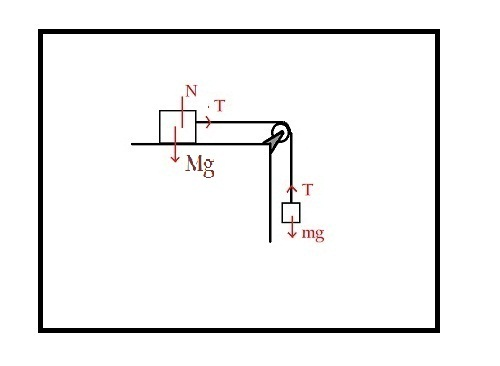
\includegraphics[width=5in]{../24/CH5/EX5.5/Example5_5_FBD.jpg}
\caption{Sample Problem 5}
\end{figure}

\vspace*{10mm}
check Appendix \ref{AP:272} for dependency: {\begin{alltt} \hspace{2mm} degree_rad.sci \end{alltt}}

\vspace*{10mm}
\curlable{Exa~5.6}
\begin{code}
\tcaption{Sample Problem 6}
\begin{verbatim}
Sample Problem 6
\end{verbatim}
\lstinputlisting{../24/CH5/EX5.6/Example5_6.sce}
\end{code}

\vspace*{10mm}
\curlable{Fig~5.6}
\begin{figure}
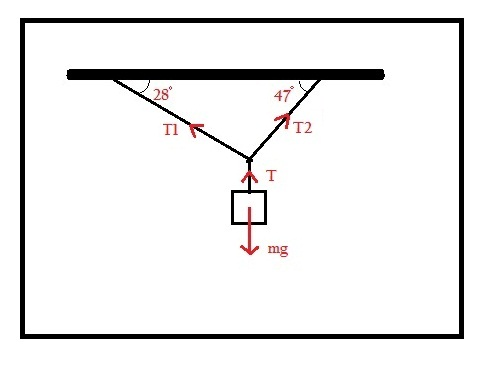
\includegraphics[width=5in]{../24/CH5/EX5.6/Example5_6_FBD.jpg}
\caption{Sample Problem 6}
\end{figure}

\vspace*{10mm}
check Appendix \ref{AP:272} for dependency: {\begin{alltt} \hspace{2mm} degree_rad.sci \end{alltt}}

\vspace*{10mm}
\curlable{Exa~5.7}
\begin{code}
\tcaption{Sample Problem 7}
\begin{verbatim}
Sample Problem 7
\end{verbatim}
\lstinputlisting{../24/CH5/EX5.7/Example5_7.sce}
\end{code}

\vspace*{10mm}
\curlable{Fig~5.7}
\begin{figure}
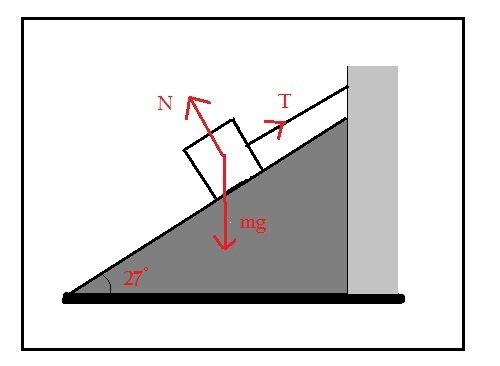
\includegraphics[width=5in]{../24/CH5/EX5.7/Example5_7_FBD.jpg}
\caption{Sample Problem 7}
\end{figure}

\vspace*{10mm}
\vspace*{10mm}
\curlable{Exa~5.8}
\begin{code}
\tcaption{Sample Problem 8}
\begin{verbatim}
Sample Problem 8
\end{verbatim}
\lstinputlisting{../24/CH5/EX5.8/Example5_8.sce}
\end{code}

\vspace*{10mm}
\curlable{Fig~5.8}
\begin{figure}
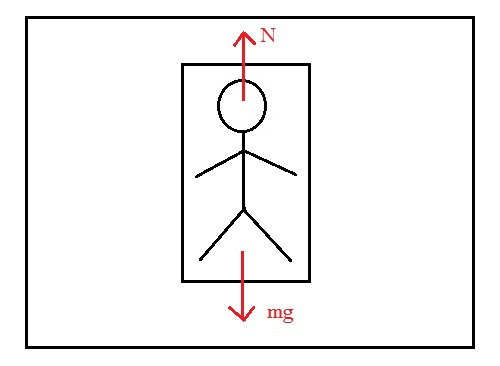
\includegraphics[width=5in]{../24/CH5/EX5.8/Example5_8_FBD.jpg}
\caption{Sample Problem 8}
\end{figure}

\vspace*{10mm}
\vspace*{10mm}
\curlable{Exa~5.9}
\begin{code}
\tcaption{Sample Problem 9}
\begin{verbatim}
Sample Problem 9
\end{verbatim}
\lstinputlisting{../24/CH5/EX5.9/Example5_9.sce}
\end{code}

\vspace*{10mm}
\curlable{Fig~5.9}
\begin{figure}
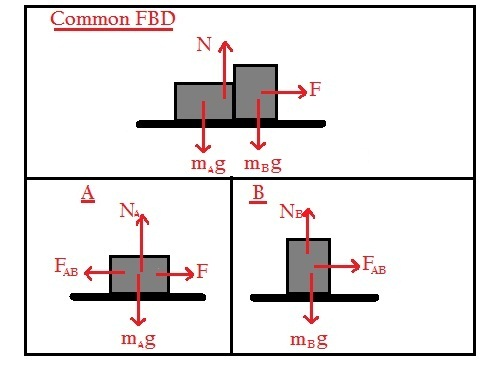
\includegraphics[width=5in]{../24/CH5/EX5.9/Example5_9_FBD.jpg}
\caption{Sample Problem 9}
\end{figure}

\vspace*{10mm}
\chapter{Force and Motion ll}

\vspace*{10mm}
\curlable{Exa~6.1}
\begin{code}
\tcaption{Sample Problem 1}
\begin{verbatim}
Sample Problem 1
\end{verbatim}
\lstinputlisting{../24/CH6/EX6.1/Example6_1.sce}
\end{code}

\vspace*{10mm}
check Appendix \ref{AP:272} for dependency: {\begin{alltt} \hspace{2mm} degree_rad.sci \end{alltt}}

\vspace*{10mm}
\curlable{Exa~6.2}
\begin{code}
\tcaption{Sample Problem 2}
\begin{verbatim}
Sample Problem 2
\end{verbatim}
\lstinputlisting{../24/CH6/EX6.2/Example6_2.sce}
\end{code}

\vspace*{10mm}
\curlable{Fig~6.2}
\begin{figure}
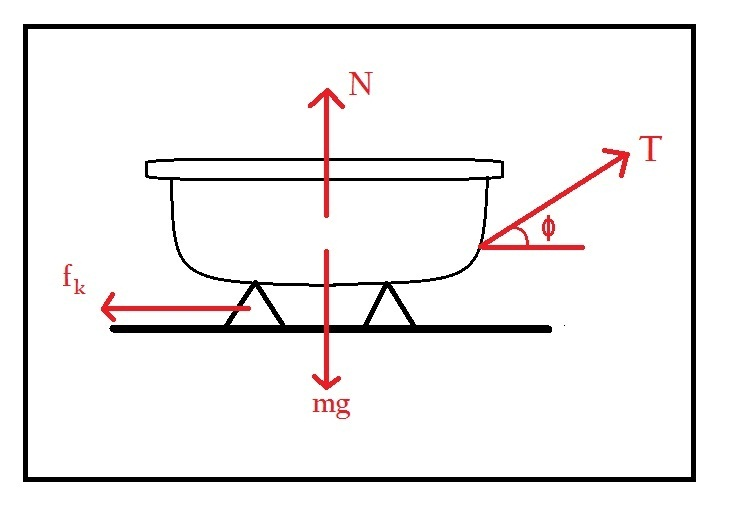
\includegraphics[width=5in]{../24/CH6/EX6.2/Example6_2_FBD.jpg}
\caption{Sample Problem 2}
\end{figure}

\vspace*{10mm}
check Appendix \ref{AP:272} for dependency: {\begin{alltt} \hspace{2mm} degree_rad.sci \end{alltt}}

\vspace*{10mm}
\curlable{Exa~6.3}
\begin{code}
\tcaption{Sample Problem 3}
\begin{verbatim}
Sample Problem 3
\end{verbatim}
\lstinputlisting{../24/CH6/EX6.3/Example6_3.sce}
\end{code}

\vspace*{10mm}
\curlable{Fig~6.3}
\begin{figure}
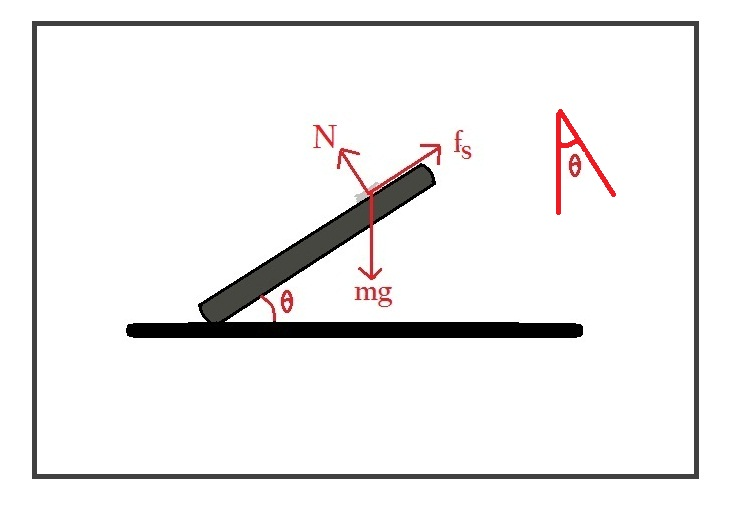
\includegraphics[width=5in]{../24/CH6/EX6.3/Example6_3_FBD.jpg}
\caption{Sample Problem 3}
\end{figure}

\vspace*{10mm}
\vspace*{10mm}
\curlable{Exa~6.4}
\begin{code}
\tcaption{Sample Problem 4}
\begin{verbatim}
Sample Problem 4
\end{verbatim}
\lstinputlisting{../24/CH6/EX6.4/Example6_4.sce}
\end{code}

\vspace*{10mm}
\vspace*{10mm}
\curlable{Exa~6.5}
\begin{code}
\tcaption{Sample Problem 5}
\begin{verbatim}
Sample Problem 5
\end{verbatim}
\lstinputlisting{../24/CH6/EX6.5/Example6_5.sce}
\end{code}

\vspace*{10mm}
\vspace*{10mm}
\curlable{Exa~6.6}
\begin{code}
\tcaption{Sample Problem 6}
\begin{verbatim}
Sample Problem 6
\end{verbatim}
\lstinputlisting{../24/CH6/EX6.6/Example6_6.sce}
\end{code}

\vspace*{10mm}
\vspace*{10mm}
\curlable{Exa~6.7}
\begin{code}
\tcaption{Sample Problem 7}
\begin{verbatim}
Sample Problem 7
\end{verbatim}
\lstinputlisting{../24/CH6/EX6.7/Example6_7.sce}
\end{code}

\vspace*{10mm}
\vspace*{10mm}
\curlable{Exa~6.8}
\begin{code}
\tcaption{Sample Problem 8}
\begin{verbatim}
Sample Problem 8
\end{verbatim}
\lstinputlisting{../24/CH6/EX6.8/Example6_8.sce}
\end{code}

\vspace*{10mm}
\curlable{Fig~6.8}
\begin{figure}
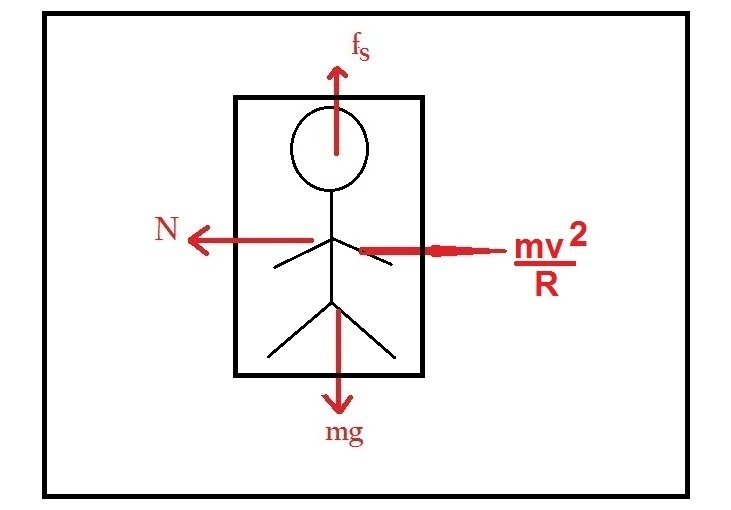
\includegraphics[width=5in]{../24/CH6/EX6.8/Example6_8_FBD.jpg}
\caption{Sample Problem 8}
\end{figure}

\vspace*{10mm}
\vspace*{10mm}
\curlable{Exa~6.9}
\begin{code}
\tcaption{Sample Problem 9}
\begin{verbatim}
Sample Problem 9
\end{verbatim}
\lstinputlisting{../24/CH6/EX6.9/Example6_9.sce}
\end{code}

\vspace*{10mm}
\curlable{Fig~6.9}
\begin{figure}
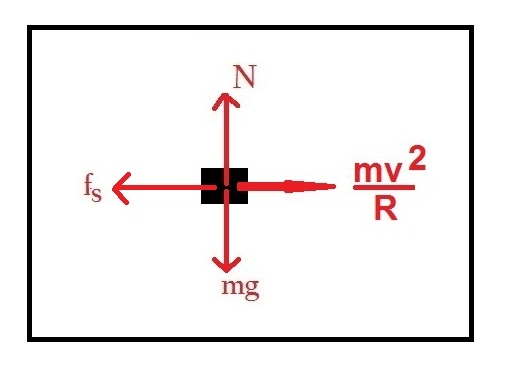
\includegraphics[width=5in]{../24/CH6/EX6.9/Example6_9_FBD.jpg}
\caption{Sample Problem 9}
\end{figure}

\vspace*{10mm}
\chapter{Kinetic Energy and Work}

check Appendix \ref{AP:272} for dependency: {\begin{alltt} \hspace{2mm} degree_rad.sci \end{alltt}}

\vspace*{10mm}
\curlable{Exa~7.1}
\begin{code}
\tcaption{Sample Problem 1}
\begin{verbatim}
Sample Problem 1
\end{verbatim}
\lstinputlisting{../24/CH7/EX7.1/Example7_1.sce}
\end{code}

\vspace*{10mm}
check Appendix \ref{AP:272} for dependency: {\begin{alltt} \hspace{2mm} degree_rad.sci \end{alltt}}

\vspace*{10mm}
\curlable{Exa~7.2}
\begin{code}
\tcaption{Sample Problem 2}
\begin{verbatim}
Sample Problem 2
\end{verbatim}
\lstinputlisting{../24/CH7/EX7.2/Example7_2.sce}
\end{code}

\vspace*{10mm}
\vspace*{10mm}
\curlable{Exa~7.3}
\begin{code}
\tcaption{Sample Problem 3}
\begin{verbatim}
Sample Problem 3
\end{verbatim}
\lstinputlisting{../24/CH7/EX7.3/Example7_3.sce}
\end{code}

\vspace*{10mm}
\vspace*{10mm}
\curlable{Exa~7.4}
\begin{code}
\tcaption{Sample Problem 4}
\begin{verbatim}
Sample Problem 4
\end{verbatim}
\lstinputlisting{../24/CH7/EX7.4/Example7_4.sce}
\end{code}

\vspace*{10mm}
\vspace*{10mm}
\curlable{Exa~7.5}
\begin{code}
\tcaption{Sample Problem 5}
\begin{verbatim}
Sample Problem 5
\end{verbatim}
\lstinputlisting{../24/CH7/EX7.5/Example7_5.sce}
\end{code}

\vspace*{10mm}
\vspace*{10mm}
\curlable{Exa~7.6}
\begin{code}
\tcaption{Sample Problem 6}
\begin{verbatim}
Sample Problem 6
\end{verbatim}
\lstinputlisting{../24/CH7/EX7.6/Example7_6.sce}
\end{code}

\vspace*{10mm}
\curlable{Fig~7.6}
\begin{figure}
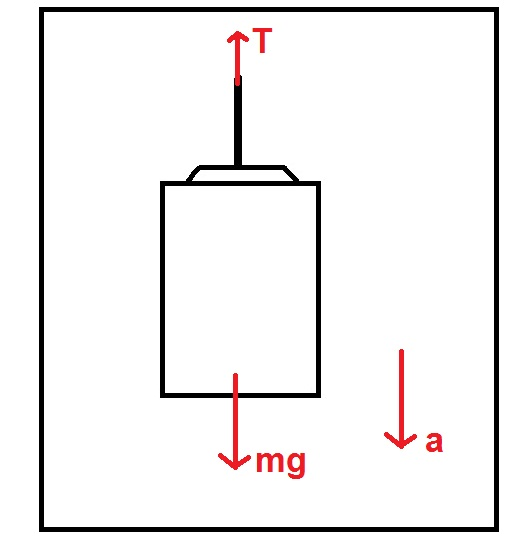
\includegraphics[width=5in]{../24/CH7/EX7.6/Example7_6_FBD.jpg}
\caption{Sample Problem 6}
\end{figure}

\vspace*{10mm}
\vspace*{10mm}
\curlable{Exa~7.7}
\begin{code}
\tcaption{Sample Problem 7}
\begin{verbatim}
Sample Problem 7
\end{verbatim}
\lstinputlisting{../24/CH7/EX7.7/Example7_7.sce}
\end{code}

\vspace*{10mm}
\vspace*{10mm}
\curlable{Exa~7.8}
\begin{code}
\tcaption{Sample Problem 8}
\begin{verbatim}
Sample Problem 8
\end{verbatim}
\lstinputlisting{../24/CH7/EX7.8/Example7_8.sce}
\end{code}

\vspace*{10mm}
\vspace*{10mm}
\curlable{Exa~7.9}
\begin{code}
\tcaption{Sample Problem 9}
\begin{verbatim}
Sample Problem 9
\end{verbatim}
\lstinputlisting{../24/CH7/EX7.9/Example7_9.sce}
\end{code}

\vspace*{10mm}
check Appendix \ref{AP:272} for dependency: {\begin{alltt} \hspace{2mm} degree_rad.sci \end{alltt}}

\vspace*{10mm}
\curlable{Exa~7.10}
\begin{code}
\tcaption{Sample Problem 10}
\begin{verbatim}
Sample Problem 10
\end{verbatim}
\lstinputlisting{../24/CH7/EX7.10/Example7_10.sce}
\end{code}

\vspace*{10mm}
\chapter{Potential and Conservation of Energy}

\vspace*{10mm}
\curlable{Exa~8.1}
\begin{code}
\tcaption{Sample Problem 1}
\begin{verbatim}
Sample Problem 1
\end{verbatim}
\lstinputlisting{../24/CH8/EX8.1/Example8_1.sce}
\end{code}

\vspace*{10mm}
\vspace*{10mm}
\curlable{Exa~8.2}
\begin{code}
\tcaption{Sample Problem 2}
\begin{verbatim}
Sample Problem 2
\end{verbatim}
\lstinputlisting{../24/CH8/EX8.2/Example8_2.sce}
\end{code}

\vspace*{10mm}
\vspace*{10mm}
\curlable{Exa~8.3}
\begin{code}
\tcaption{Sample Problem 3}
\begin{verbatim}
Sample Problem 3
\end{verbatim}
\lstinputlisting{../24/CH8/EX8.3/Example8_3.sce}
\end{code}

\vspace*{10mm}
\vspace*{10mm}
\curlable{Exa~8.4}
\begin{code}
\tcaption{Sample Problem 4}
\begin{verbatim}
Sample Problem 4
\end{verbatim}
\lstinputlisting{../24/CH8/EX8.4/Example8_4.sce}
\end{code}

\vspace*{10mm}
\vspace*{10mm}
\curlable{Exa~8.5}
\begin{code}
\tcaption{Sample Problem 5}
\begin{verbatim}
Sample Problem 5
\end{verbatim}
\lstinputlisting{../24/CH8/EX8.5/Example8_5.sce}
\end{code}

\vspace*{10mm}
\vspace*{10mm}
\curlable{Exa~8.6}
\begin{code}
\tcaption{Sample Problem 6}
\begin{verbatim}
Sample Problem 6
\end{verbatim}
\lstinputlisting{../24/CH8/EX8.6/Example8_6.sce}
\end{code}

\vspace*{10mm}
\vspace*{10mm}
\curlable{Exa~8.7}
\begin{code}
\tcaption{Sample Problem 7}
\begin{verbatim}
Sample Problem 7
\end{verbatim}
\lstinputlisting{../24/CH8/EX8.7/Example8_7.sce}
\end{code}

\vspace*{10mm}
\vspace*{10mm}
\curlable{Exa~8.8}
\begin{code}
\tcaption{Sample Problem 8}
\begin{verbatim}
Sample Problem 8
\end{verbatim}
\lstinputlisting{../24/CH8/EX8.8/Example8_8.sce}
\end{code}

\vspace*{10mm}
\chapter{System of Particles}

check Appendix \ref{AP:272} for dependency: {\begin{alltt} \hspace{2mm} degree_rad.sci \end{alltt}}

\vspace*{10mm}
\curlable{Exa~9.1}
\begin{code}
\tcaption{Sample Problem 1}
\begin{verbatim}
Sample Problem 1
\end{verbatim}
\lstinputlisting{../24/CH9/EX9.1/Example9_1.sce}
\end{code}

\vspace*{10mm}
\curlable{Fig~9.1}
\begin{figure}
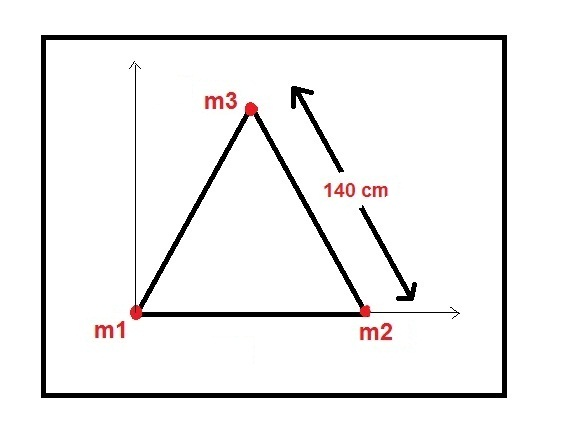
\includegraphics[width=5in]{../24/CH9/EX9.1/Example9_1_figure.jpg}
\caption{Sample Problem 1}
\end{figure}

\vspace*{10mm}
\vspace*{10mm}
\curlable{Exa~9.2}
\begin{code}
\tcaption{Sample Problem 2}
\begin{verbatim}
Sample Problem 2
\end{verbatim}
\lstinputlisting{../24/CH9/EX9.2/Example9_2.sce}
\end{code}

\vspace*{10mm}
check Appendix \ref{AP:272} for dependency: {\begin{alltt} \hspace{2mm} degree_rad.sci \end{alltt}}

\vspace*{10mm}
\curlable{Exa~9.3}
\begin{code}
\tcaption{Sample Problem 3}
\begin{verbatim}
Sample Problem 3
\end{verbatim}
\lstinputlisting{../24/CH9/EX9.3/Example9_3.sce}
\end{code}

\vspace*{10mm}
check Appendix \ref{AP:272} for dependency: {\begin{alltt} \hspace{2mm} degree_rad.sci \end{alltt}}

\vspace*{10mm}
\curlable{Exa~9.4}
\begin{code}
\tcaption{Sample Problem 4}
\begin{verbatim}
Sample Problem 4
\end{verbatim}
\lstinputlisting{../24/CH9/EX9.4/Example9_4.sce}
\end{code}

\vspace*{10mm}
\vspace*{10mm}
\curlable{Exa~9.5}
\begin{code}
\tcaption{Sample Problem 5}
\begin{verbatim}
Sample Problem 5
\end{verbatim}
\lstinputlisting{../24/CH9/EX9.5/Example9_5.sce}
\end{code}

\vspace*{10mm}
\vspace*{10mm}
\curlable{Exa~9.6}
\begin{code}
\tcaption{Sample Problem 6}
\begin{verbatim}
Sample Problem 6
\end{verbatim}
\lstinputlisting{../24/CH9/EX9.6/Example9_6.sce}
\end{code}

\vspace*{10mm}
check Appendix \ref{AP:272} for dependency: {\begin{alltt} \hspace{2mm} degree_rad.sci \end{alltt}}

\vspace*{10mm}
\curlable{Exa~9.7}
\begin{code}
\tcaption{Sample Problem 7}
\begin{verbatim}
Sample Problem 7
\end{verbatim}
\lstinputlisting{../24/CH9/EX9.7/Example9_7.sce}
\end{code}

\vspace*{10mm}
\vspace*{10mm}
\curlable{Exa~9.8}
\begin{code}
\tcaption{Sample Problem 8}
\begin{verbatim}
Sample Problem 8
\end{verbatim}
\lstinputlisting{../24/CH9/EX9.8/Example9_8.sce}
\end{code}

\vspace*{10mm}
check Appendix \ref{AP:272} for dependency: {\begin{alltt} \hspace{2mm} degree_rad.sci \end{alltt}}

\vspace*{10mm}
\curlable{Exa~9.9}
\begin{code}
\tcaption{Sample Problem 9}
\begin{verbatim}
Sample Problem 9
\end{verbatim}
\lstinputlisting{../24/CH9/EX9.9/Example9_9.sce}
\end{code}

\vspace*{10mm}
\chapter{Collisions}

check Appendix \ref{AP:272} for dependency: {\begin{alltt} \hspace{2mm} degree_rad.sci \end{alltt}}

\vspace*{10mm}
\curlable{Exa~10.1}
\begin{code}
\tcaption{Sample Problem 1}
\begin{verbatim}
Sample Problem 1
\end{verbatim}
\lstinputlisting{../24/CH10/EX10.1/Example10_1.sce}
\end{code}

\vspace*{10mm}
\vspace*{10mm}
\curlable{Exa~10.2}
\begin{code}
\tcaption{Sample Problem 2}
\begin{verbatim}
Sample Problem 2
\end{verbatim}
\lstinputlisting{../24/CH10/EX10.2/Example10_2.sce}
\end{code}

\vspace*{10mm}
\vspace*{10mm}
\curlable{Exa~10.3}
\begin{code}
\tcaption{Sample Problem 3}
\begin{verbatim}
Sample Problem 3
\end{verbatim}
\lstinputlisting{../24/CH10/EX10.3/Example10_3.sce}
\end{code}

\vspace*{10mm}
check Appendix \ref{AP:280} for dependency: {\begin{alltt} \hspace{2mm} collision.sci \end{alltt}}

\vspace*{10mm}
\curlable{Exa~10.4}
\begin{code}
\tcaption{Sample Problem 4}
\begin{verbatim}
Sample Problem 4
\end{verbatim}
\lstinputlisting{../24/CH10/EX10.4/Example10_4.sce}
\end{code}

\vspace*{10mm}
\vspace*{10mm}
\curlable{Exa~10.5}
\begin{code}
\tcaption{Sample Problem 5}
\begin{verbatim}
Sample Problem 5
\end{verbatim}
\lstinputlisting{../24/CH10/EX10.5/Example10_5.sce}
\end{code}

\vspace*{10mm}
\chapter{Rotation}

\vspace*{10mm}
\curlable{Exa~11.1}
\begin{code}
\tcaption{Sample Problem 1}
\begin{verbatim}
Sample Problem 1
\end{verbatim}
\lstinputlisting{../24/CH11/EX11.1/Example11_1.sce}
\end{code}

\vspace*{10mm}
\curlable{Fig~11.1}
\begin{figure}
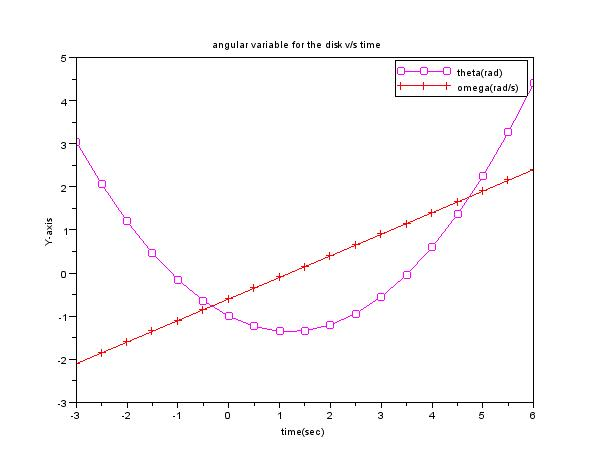
\includegraphics[width=5in]{../24/CH11/EX11.1/Example11_1_graph.jpg}
\caption{Sample Problem 1}
\end{figure}

\vspace*{10mm}
\vspace*{10mm}
\curlable{Exa~11.2}
\begin{code}
\tcaption{Sample Problem 2}
\begin{verbatim}
Sample Problem 2
\end{verbatim}
\lstinputlisting{../24/CH11/EX11.2/Example11_2.sce}
\end{code}

\vspace*{10mm}
\vspace*{10mm}
\curlable{Exa~11.3}
\begin{code}
\tcaption{Sample Problem 3}
\begin{verbatim}
Sample Problem 3
\end{verbatim}
\lstinputlisting{../24/CH11/EX11.3/Example11_3.sce}
\end{code}

\vspace*{10mm}
\vspace*{10mm}
\curlable{Exa~11.4}
\begin{code}
\tcaption{Sample Problem 4}
\begin{verbatim}
Sample Problem 4
\end{verbatim}
\lstinputlisting{../24/CH11/EX11.4/Example11_4.sce}
\end{code}

\vspace*{10mm}
\vspace*{10mm}
\curlable{Exa~11.6}
\begin{code}
\tcaption{Sample Problem 6}
\begin{verbatim}
Sample Problem 6
\end{verbatim}
\lstinputlisting{../24/CH11/EX11.6/Example11_6.sce}
\end{code}

\vspace*{10mm}
\vspace*{10mm}
\curlable{Exa~11.7}
\begin{code}
\tcaption{Sample Problem 7}
\begin{verbatim}
Sample Problem 7
\end{verbatim}
\lstinputlisting{../24/CH11/EX11.7/Example11_7.sce}
\end{code}

\vspace*{10mm}
\curlable{Fig~11.7}
\begin{figure}
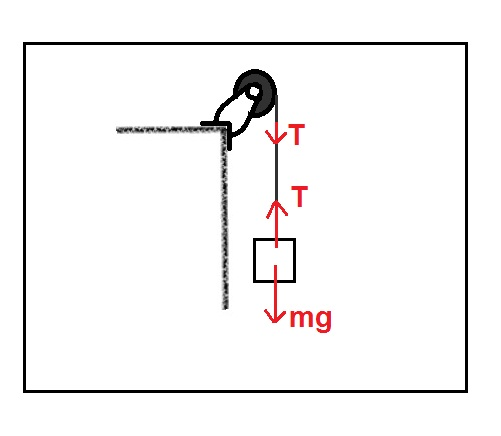
\includegraphics[width=5in]{../24/CH11/EX11.7/Example11_7_FBD.jpg}
\caption{Sample Problem 7}
\end{figure}

\vspace*{10mm}
\vspace*{10mm}
\curlable{Exa~11.8}
\begin{code}
\tcaption{Sample Problem 8}
\begin{verbatim}
Sample Problem 8
\end{verbatim}
\lstinputlisting{../24/CH11/EX11.8/Example11_8.sce}
\end{code}

\vspace*{10mm}
check Appendix \ref{AP:281} for dependency: {\begin{alltt} \hspace{2mm} Example11_7.sce \end{alltt}}

\vspace*{10mm}
\curlable{Exa~11.9}
\begin{code}
\tcaption{Sample Problem 9}
\begin{verbatim}
Sample Problem 9
\end{verbatim}
\lstinputlisting{../24/CH11/EX11.9/Example11_9.sce}
\end{code}

\vspace*{10mm}
\vspace*{10mm}
\curlable{Exa~11.10}
\begin{code}
\tcaption{Sample Problem 10}
\begin{verbatim}
Sample Problem 10
\end{verbatim}
\lstinputlisting{../24/CH11/EX11.10/Example11_10.sce}
\end{code}

\vspace*{10mm}
\chapter{Rolling Torque and Angular Momentum}

\vspace*{10mm}
\curlable{Exa~12.1}
\begin{code}
\tcaption{Sample Problem 1}
\begin{verbatim}
Sample Problem 1
\end{verbatim}
\lstinputlisting{../24/CH12/EX12.1/Example12_1.sce}
\end{code}

\vspace*{10mm}
check Appendix \ref{AP:272} for dependency: {\begin{alltt} \hspace{2mm} degree_rad.sci \end{alltt}}

\vspace*{10mm}
\curlable{Exa~12.2}
\begin{code}
\tcaption{Sample Problem 2}
\begin{verbatim}
Sample Problem 2
\end{verbatim}
\lstinputlisting{../24/CH12/EX12.2/Example12_2.sce}
\end{code}

\vspace*{10mm}
check Appendix \ref{AP:277} for dependency: {\begin{alltt} \hspace{2mm} cross_product.sci \end{alltt}}

check Appendix \ref{AP:272} for dependency: {\begin{alltt} \hspace{2mm} degree_rad.sci \end{alltt}}

\vspace*{10mm}
\curlable{Exa~12.3}
\begin{code}
\tcaption{Sample Problem 3}
\begin{verbatim}
Sample Problem 3
\end{verbatim}
\lstinputlisting{../24/CH12/EX12.3/Example12_3.sce}
\end{code}

\vspace*{10mm}
\vspace*{10mm}
\curlable{Exa~12.4}
\begin{code}
\tcaption{Sample Problem 4}
\begin{verbatim}
Sample Problem 4
\end{verbatim}
\lstinputlisting{../24/CH12/EX12.4/Example12_4.sce}
\end{code}

\vspace*{10mm}
\vspace*{10mm}
\curlable{Exa~12.6}
\begin{code}
\tcaption{Sample Problem 6}
\begin{verbatim}
Sample Problem 6
\end{verbatim}
\lstinputlisting{../24/CH12/EX12.6/Example12_6.sce}
\end{code}

\vspace*{10mm}
\vspace*{10mm}
\curlable{Exa~12.7}
\begin{code}
\tcaption{Sample Problem 7}
\begin{verbatim}
Sample Problem 7
\end{verbatim}
\lstinputlisting{../24/CH12/EX12.7/Example12_7.sce}
\end{code}

\vspace*{10mm}
\vspace*{10mm}
\curlable{Exa~12.8}
\begin{code}
\tcaption{Sample Problem 8}
\begin{verbatim}
Sample Problem 8
\end{verbatim}
\lstinputlisting{../24/CH12/EX12.8/Example12_8.sce}
\end{code}

\vspace*{10mm}
\vspace*{10mm}
\curlable{Exa~12.9}
\begin{code}
\tcaption{Sample Problem 9}
\begin{verbatim}
Sample Problem 9
\end{verbatim}
\lstinputlisting{../24/CH12/EX12.9/Example12_9.sce}
\end{code}

\vspace*{10mm}
\chapter{Equilibrium and Elasticity}

\vspace*{10mm}
\curlable{Exa~13.1}
\begin{code}
\tcaption{Sample Problem 1}
\begin{verbatim}
Sample Problem 1
\end{verbatim}
\lstinputlisting{../24/CH13/EX13.1/Example13_1.sce}
\end{code}

\vspace*{10mm}
\curlable{Fig~13.1}
\begin{figure}
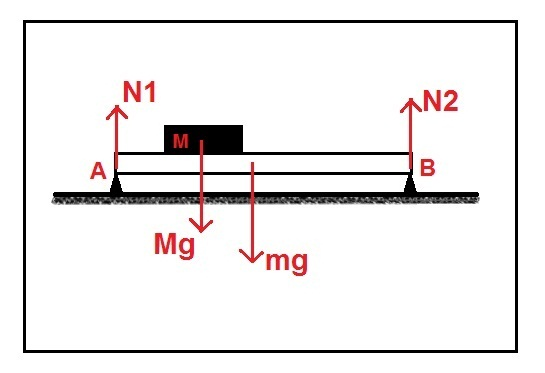
\includegraphics[width=5in]{../24/CH13/EX13.1/Example13_1_FBD.jpg}
\caption{Sample Problem 1}
\end{figure}

\vspace*{10mm}
\vspace*{10mm}
\curlable{Exa~13.2}
\begin{code}
\tcaption{Sample Problem 2}
\begin{verbatim}
Sample Problem 2
\end{verbatim}
\lstinputlisting{../24/CH13/EX13.2/Example13_2.sce}
\end{code}

\vspace*{10mm}
\curlable{Fig~13.2}
\begin{figure}
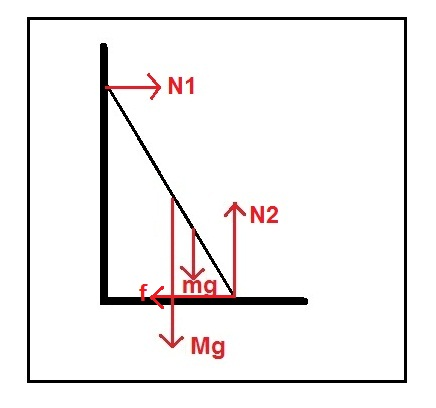
\includegraphics[width=5in]{../24/CH13/EX13.2/Example13_2_FBD.jpg}
\caption{Sample Problem 2}
\end{figure}

\vspace*{10mm}
\vspace*{10mm}
\curlable{Exa~13.3}
\begin{code}
\tcaption{Sample Problem 3}
\begin{verbatim}
Sample Problem 3
\end{verbatim}
\lstinputlisting{../24/CH13/EX13.3/Example13_3.sce}
\end{code}

\vspace*{10mm}
\curlable{Fig~13.3}
\begin{figure}
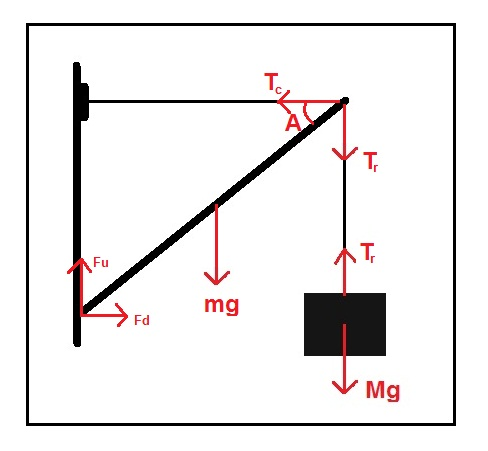
\includegraphics[width=5in]{../24/CH13/EX13.3/Example13_3_FBD.jpg}
\caption{Sample Problem 3}
\end{figure}

\vspace*{10mm}
\vspace*{10mm}
\curlable{Exa~13.4}
\begin{code}
\tcaption{Sample Problem 4}
\begin{verbatim}
Sample Problem 4
\end{verbatim}
\lstinputlisting{../24/CH13/EX13.4/Example13_4.sce}
\end{code}

\vspace*{10mm}
\curlable{Fig~13.4}
\begin{figure}
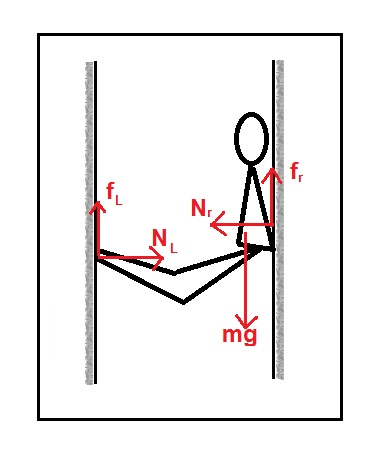
\includegraphics[width=5in]{../24/CH13/EX13.4/Example13_4_FBD.jpg}
\caption{Sample Problem 4}
\end{figure}

\vspace*{10mm}
\vspace*{10mm}
\curlable{Exa~13.5}
\begin{code}
\tcaption{Sample Problem 5}
\begin{verbatim}
Sample Problem 5
\end{verbatim}
\lstinputlisting{../24/CH13/EX13.5/Example13_5.sce}
\end{code}

\vspace*{10mm}
\vspace*{10mm}
\curlable{Exa~13.6}
\begin{code}
\tcaption{Sample Problem 6}
\begin{verbatim}
Sample Problem 6
\end{verbatim}
\lstinputlisting{../24/CH13/EX13.6/Example13_6.sce}
\end{code}

\vspace*{10mm}
\chapter{Gravitation}

check Appendix \ref{AP:273} for dependency: {\begin{alltt} \hspace{2mm} Gravitation.sci \end{alltt}}

\vspace*{10mm}
\curlable{Exa~14.1}
\begin{code}
\tcaption{Sample Problem 1}
\begin{verbatim}
Sample Problem 1
\end{verbatim}
\lstinputlisting{../24/CH14/EX14.1/Example14_1.sce}
\end{code}

\vspace*{10mm}
check Appendix \ref{AP:273} for dependency: {\begin{alltt} \hspace{2mm} Gravitation.sci \end{alltt}}

check Appendix \ref{AP:272} for dependency: {\begin{alltt} \hspace{2mm} degree_rad.sci \end{alltt}}

\vspace*{10mm}
\curlable{Exa~14.2}
\begin{code}
\tcaption{Sample Problem 2}
\begin{verbatim}
Sample Problem 2
\end{verbatim}
\lstinputlisting{../24/CH14/EX14.2/Example14_2.sce}
\end{code}

\vspace*{10mm}
\vspace*{10mm}
\curlable{Exa~14.3.a}
\begin{code}
\tcaption{Sample Problem 3a}
\begin{verbatim}
Sample Problem 3a
\end{verbatim}
\lstinputlisting{../24/CH14/EX14.3.a/Example14_3a.sce}
\end{code}

\vspace*{10mm}
check Appendix \ref{AP:273} for dependency: {\begin{alltt} \hspace{2mm} Gravitation.sci \end{alltt}}

\vspace*{10mm}
\curlable{Exa~14.3.b}
\begin{code}
\tcaption{Sample Problem 3b}
\begin{verbatim}
Sample Problem 3b
\end{verbatim}
\lstinputlisting{../24/CH14/EX14.3.b/Example14_3b.sce}
\end{code}

\vspace*{10mm}
check Appendix \ref{AP:273} for dependency: {\begin{alltt} \hspace{2mm} Gravitation.sci \end{alltt}}

check Appendix \ref{AP:273} for dependency: {\begin{alltt} \hspace{2mm} Gravitation.sci \end{alltt}}

\vspace*{10mm}
\curlable{Exa~14.5}
\begin{code}
\tcaption{Sample Problem 5}
\begin{verbatim}
Sample Problem 5
\end{verbatim}
\lstinputlisting{../24/CH14/EX14.5/Example14_5.sce}
\end{code}

\vspace*{10mm}
check Appendix \ref{AP:273} for dependency: {\begin{alltt} \hspace{2mm} Gravitation.sci \end{alltt}}

\vspace*{10mm}
\curlable{Exa~14.6}
\begin{code}
\tcaption{Sample Problem 6}
\begin{verbatim}
Sample Problem 6
\end{verbatim}
\lstinputlisting{../24/CH14/EX14.6/Example14_6.sce}
\end{code}

\vspace*{10mm}
check Appendix \ref{AP:273} for dependency: {\begin{alltt} \hspace{2mm} Gravitation.sci \end{alltt}}

\vspace*{10mm}
\curlable{Exa~14.7}
\begin{code}
\tcaption{Sample Problem 7}
\begin{verbatim}
Sample Problem 7
\end{verbatim}
\lstinputlisting{../24/CH14/EX14.7/Example14_7.sce}
\end{code}

\vspace*{10mm}
check Appendix \ref{AP:273} for dependency: {\begin{alltt} \hspace{2mm} Gravitation.sci \end{alltt}}

\vspace*{10mm}
\curlable{Exa~14.8}
\begin{code}
\tcaption{Sample Problem 8}
\begin{verbatim}
Sample Problem 8
\end{verbatim}
\lstinputlisting{../24/CH14/EX14.8/Example14_8.sce}
\end{code}

\vspace*{10mm}
\chapter{Fluids}

\vspace*{10mm}
\curlable{Exa~15.1}
\begin{code}
\tcaption{Sample Problem 1}
\begin{verbatim}
Sample Problem 1
\end{verbatim}
\lstinputlisting{../24/CH15/EX15.1/Example15_1.sce}
\end{code}

\vspace*{10mm}
\vspace*{10mm}
\curlable{Exa~15.2}
\begin{code}
\tcaption{Sample Problem 2}
\begin{verbatim}
Sample Problem 2
\end{verbatim}
\lstinputlisting{../24/CH15/EX15.2/Example15_2.sce}
\end{code}

\vspace*{10mm}
\vspace*{10mm}
\curlable{Exa~15.3}
\begin{code}
\tcaption{Sample Problem 3}
\begin{verbatim}
Sample Problem 3
\end{verbatim}
\lstinputlisting{../24/CH15/EX15.3/Example15_3.sce}
\end{code}

\vspace*{10mm}
\vspace*{10mm}
\curlable{Exa~15.4}
\begin{code}
\tcaption{Sample Problem 4}
\begin{verbatim}
Sample Problem 4
\end{verbatim}
\lstinputlisting{../24/CH15/EX15.4/Example15_4.sce}
\end{code}

\vspace*{10mm}
\vspace*{10mm}
\curlable{Exa~15.5}
\begin{code}
\tcaption{Sample Problem 5}
\begin{verbatim}
Sample Problem 5
\end{verbatim}
\lstinputlisting{../24/CH15/EX15.5/Example15_5.sce}
\end{code}

\vspace*{10mm}
\vspace*{10mm}
\curlable{Exa~15.6}
\begin{code}
\tcaption{Sample Problem 6}
\begin{verbatim}
Sample Problem 6
\end{verbatim}
\lstinputlisting{../24/CH15/EX15.6/Example15_6.sce}
\end{code}

\vspace*{10mm}
check Appendix \ref{AP:282} for dependency: {\begin{alltt} \hspace{2mm} Bernauli.sci \end{alltt}}

\vspace*{10mm}
\curlable{Exa~15.7}
\begin{code}
\tcaption{Sample Problem 7}
\begin{verbatim}
Sample Problem 7
\end{verbatim}
\lstinputlisting{../24/CH15/EX15.7/Example15_7.sce}
\end{code}

\vspace*{10mm}
check Appendix \ref{AP:282} for dependency: {\begin{alltt} \hspace{2mm} Bernauli.sci \end{alltt}}

\vspace*{10mm}
\curlable{Exa~15.8}
\begin{code}
\tcaption{Sample Problem 8}
\begin{verbatim}
Sample Problem 8
\end{verbatim}
\lstinputlisting{../24/CH15/EX15.8/Example15_8.sce}
\end{code}

\vspace*{10mm}
\chapter{Oscillation}

\vspace*{10mm}
\curlable{Exa~16.1}
\begin{code}
\tcaption{Sample Problem 1}
\begin{verbatim}
Sample Problem 1
\end{verbatim}
\lstinputlisting{../24/CH16/EX16.1/Example16_1.sce}
\end{code}

\vspace*{10mm}
\vspace*{10mm}
\curlable{Exa~16.2}
\begin{code}
\tcaption{Sample Problem 2}
\begin{verbatim}
Sample Problem 2
\end{verbatim}
\lstinputlisting{../24/CH16/EX16.2/Example16_2.sce}
\end{code}

\vspace*{10mm}
\vspace*{10mm}
\curlable{Exa~16.3}
\begin{code}
\tcaption{Sample Problem 3}
\begin{verbatim}
Sample Problem 3
\end{verbatim}
\lstinputlisting{../24/CH16/EX16.3/Example16_3.sce}
\end{code}

\vspace*{10mm}
\vspace*{10mm}
\curlable{Exa~16.4}
\begin{code}
\tcaption{Sample Problem 4}
\begin{verbatim}
Sample Problem 4
\end{verbatim}
\lstinputlisting{../24/CH16/EX16.4/Example16_4.sce}
\end{code}

\vspace*{10mm}
\vspace*{10mm}
\curlable{Exa~16.5}
\begin{code}
\tcaption{Sample Problem 5}
\begin{verbatim}
Sample Problem 5
\end{verbatim}
\lstinputlisting{../24/CH16/EX16.5/Example16_5.sce}
\end{code}

\vspace*{10mm}
\vspace*{10mm}
\curlable{Exa~16.6}
\begin{code}
\tcaption{Sample Problem 6}
\begin{verbatim}
Sample Problem 6
\end{verbatim}
\lstinputlisting{../24/CH16/EX16.6/Example16_6.sce}
\end{code}

\vspace*{10mm}
\curlable{Fig~16.6}
\begin{figure}
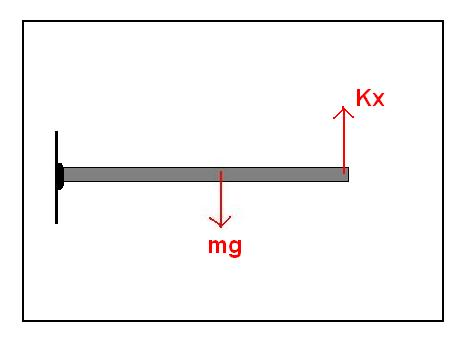
\includegraphics[width=5in]{../24/CH16/EX16.6/Example16_6_FBD.JPG}
\caption{Sample Problem 6}
\end{figure}

\vspace*{10mm}
\vspace*{10mm}
\curlable{Exa~16.7}
\begin{code}
\tcaption{Sample Problem 7}
\begin{verbatim}
Sample Problem 7
\end{verbatim}
\lstinputlisting{../24/CH16/EX16.7/Example16_7.sce}
\end{code}

\vspace*{10mm}
\chapter{Waves l}

\vspace*{10mm}
\curlable{Exa~17.1}
\begin{code}
\tcaption{Sample Problem 1}
\begin{verbatim}
Sample Problem 1
\end{verbatim}
\lstinputlisting{../24/CH17/EX17.1/Example17_1.sce}
\end{code}

\vspace*{10mm}
check Appendix \ref{AP:283} for dependency: {\begin{alltt} \hspace{2mm} Example17_1.sce \end{alltt}}

\vspace*{10mm}
\curlable{Exa~17.2}
\begin{code}
\tcaption{Sample Problem 2}
\begin{verbatim}
Sample Problem 2
\end{verbatim}
\lstinputlisting{../24/CH17/EX17.2/Example17_2.sce}
\end{code}

\vspace*{10mm}
\vspace*{10mm}
\curlable{Exa~17.3}
\begin{code}
\tcaption{Sample Problem 3}
\begin{verbatim}
Sample Problem 3
\end{verbatim}
\lstinputlisting{../24/CH17/EX17.3/Example17_3.sce}
\end{code}

\vspace*{10mm}
\vspace*{10mm}
\curlable{Exa~17.4}
\begin{code}
\tcaption{Sample Problem 4}
\begin{verbatim}
Sample Problem 4
\end{verbatim}
\lstinputlisting{../24/CH17/EX17.4/Example17_4.sce}
\end{code}

\vspace*{10mm}
check Appendix \ref{AP:272} for dependency: {\begin{alltt} \hspace{2mm} degree_rad.sci \end{alltt}}

\vspace*{10mm}
\curlable{Exa~17.5}
\begin{code}
\tcaption{Sample Problem 5}
\begin{verbatim}
Sample Problem 5
\end{verbatim}
\lstinputlisting{../24/CH17/EX17.5/Example17_5.sce}
\end{code}

\vspace*{10mm}
\vspace*{10mm}
\curlable{Exa~17.6}
\begin{code}
\tcaption{Sample Problem 6}
\begin{verbatim}
Sample Problem 6
\end{verbatim}
\lstinputlisting{../24/CH17/EX17.6/Example17_6.sce}
\end{code}

\vspace*{10mm}
\vspace*{10mm}
\curlable{Exa~17.7}
\begin{code}
\tcaption{Sample Problem 7}
\begin{verbatim}
Sample Problem 7
\end{verbatim}
\lstinputlisting{../24/CH17/EX17.7/Example17_7.sce}
\end{code}

\vspace*{10mm}
\chapter{Waves ll}

check Appendix \ref{AP:272} for dependency: {\begin{alltt} \hspace{2mm} degree_rad.sci \end{alltt}}

\vspace*{10mm}
\curlable{Exa~18.1}
\begin{code}
\tcaption{Sample Problem 1}
\begin{verbatim}
Sample Problem 1
\end{verbatim}
\lstinputlisting{../24/CH18/EX18.1/Example18_1.sce}
\end{code}

\vspace*{10mm}
\vspace*{10mm}
\curlable{Exa~18.2}
\begin{code}
\tcaption{Sample Problem 2}
\begin{verbatim}
Sample Problem 2
\end{verbatim}
\lstinputlisting{../24/CH18/EX18.2/Example18_2.sce}
\end{code}

\vspace*{10mm}
\vspace*{10mm}
\curlable{Exa~18.3}
\begin{code}
\tcaption{Sample Problem 3}
\begin{verbatim}
Sample Problem 3
\end{verbatim}
\lstinputlisting{../24/CH18/EX18.3/Example18_3.sce}
\end{code}

\vspace*{10mm}
\vspace*{10mm}
\curlable{Exa~18.4}
\begin{code}
\tcaption{Sample Problem 4}
\begin{verbatim}
Sample Problem 4
\end{verbatim}
\lstinputlisting{../24/CH18/EX18.4/Example18_4.sce}
\end{code}

\vspace*{10mm}
\vspace*{10mm}
\curlable{Exa~18.5}
\begin{code}
\tcaption{Sample Problem 5}
\begin{verbatim}
Sample Problem 5
\end{verbatim}
\lstinputlisting{../24/CH18/EX18.5/Example18_5.sce}
\end{code}

\vspace*{10mm}
\vspace*{10mm}
\curlable{Exa~18.6}
\begin{code}
\tcaption{Sample Problem 6}
\begin{verbatim}
Sample Problem 6
\end{verbatim}
\lstinputlisting{../24/CH18/EX18.6/Example18_6.sce}
\end{code}

\vspace*{10mm}
\vspace*{10mm}
\curlable{Exa~18.8}
\begin{code}
\tcaption{Sample Problem 8}
\begin{verbatim}
Sample Problem 8
\end{verbatim}
\lstinputlisting{../24/CH18/EX18.8/Example18_8.sce}
\end{code}

\vspace*{10mm}
\chapter{Temprature Heat and the First Law of Thermodynamic}

\vspace*{10mm}
\curlable{Exa~19.1}
\begin{code}
\tcaption{Sample Problem 1}
\begin{verbatim}
Sample Problem 1
\end{verbatim}
\lstinputlisting{../24/CH19/EX19.1/Example19_1.sce}
\end{code}

\vspace*{10mm}
\vspace*{10mm}
\curlable{Exa~19.2}
\begin{code}
\tcaption{Sample Problem 2}
\begin{verbatim}
Sample Problem 2
\end{verbatim}
\lstinputlisting{../24/CH19/EX19.2/Example19_2.sce}
\end{code}

\vspace*{10mm}
\vspace*{10mm}
\curlable{Exa~19.3}
\begin{code}
\tcaption{Sample Problem 3}
\begin{verbatim}
Sample Problem 3
\end{verbatim}
\lstinputlisting{../24/CH19/EX19.3/Example19_3.sce}
\end{code}

\vspace*{10mm}
\vspace*{10mm}
\curlable{Exa~19.4}
\begin{code}
\tcaption{Sample Problem 4}
\begin{verbatim}
Sample Problem 4
\end{verbatim}
\lstinputlisting{../24/CH19/EX19.4/Example19_4.sce}
\end{code}

\vspace*{10mm}
\vspace*{10mm}
\curlable{Exa~19.5}
\begin{code}
\tcaption{Sample Problem 5}
\begin{verbatim}
Sample Problem 5
\end{verbatim}
\lstinputlisting{../24/CH19/EX19.5/Example19_5.sce}
\end{code}

\vspace*{10mm}
\vspace*{10mm}
\curlable{Exa~19.6}
\begin{code}
\tcaption{Sample Problem 6}
\begin{verbatim}
Sample Problem 6
\end{verbatim}
\lstinputlisting{../24/CH19/EX19.6/Example19_6.sce}
\end{code}

\vspace*{10mm}
\vspace*{10mm}
\curlable{Exa~19.7}
\begin{code}
\tcaption{Sample Problem 7}
\begin{verbatim}
Sample Problem 7
\end{verbatim}
\lstinputlisting{../24/CH19/EX19.7/Example19_7.sce}
\end{code}

\vspace*{10mm}
\chapter{The Kinetic Theory of Gases}

\vspace*{10mm}
\curlable{Exa~20.1}
\begin{code}
\tcaption{Sample Problem 1}
\begin{verbatim}
Sample Problem 1
\end{verbatim}
\lstinputlisting{../24/CH20/EX20.1/Example20_1.sce}
\end{code}

\vspace*{10mm}
\vspace*{10mm}
\curlable{Exa~20.2}
\begin{code}
\tcaption{Sample Problem 2}
\begin{verbatim}
Sample Problem 2
\end{verbatim}
\lstinputlisting{../24/CH20/EX20.2/Example20_2.sce}
\end{code}

\vspace*{10mm}
\vspace*{10mm}
\curlable{Exa~20.3}
\begin{code}
\tcaption{Sample Problem 3}
\begin{verbatim}
Sample Problem 3
\end{verbatim}
\lstinputlisting{../24/CH20/EX20.3/Example20_3.sce}
\end{code}

\vspace*{10mm}
\vspace*{10mm}
\curlable{Exa~20.4}
\begin{code}
\tcaption{Sample Problem 4}
\begin{verbatim}
Sample Problem 4
\end{verbatim}
\lstinputlisting{../24/CH20/EX20.4/Example20_4.sce}
\end{code}

\vspace*{10mm}
\vspace*{10mm}
\curlable{Exa~20.5}
\begin{code}
\tcaption{Sample Problem 5}
\begin{verbatim}
Sample Problem 5
\end{verbatim}
\lstinputlisting{../24/CH20/EX20.5/Example20_5.sce}
\end{code}

\vspace*{10mm}
\vspace*{10mm}
\curlable{Exa~20.6}
\begin{code}
\tcaption{Sample Problem 6}
\begin{verbatim}
Sample Problem 6
\end{verbatim}
\lstinputlisting{../24/CH20/EX20.6/Example20_6.sce}
\end{code}

\vspace*{10mm}
\vspace*{10mm}
\curlable{Exa~20.7}
\begin{code}
\tcaption{Sample Problem 7}
\begin{verbatim}
Sample Problem 7
\end{verbatim}
\lstinputlisting{../24/CH20/EX20.7/Example20_7.sce}
\end{code}

\vspace*{10mm}
\vspace*{10mm}
\curlable{Exa~20.9}
\begin{code}
\tcaption{Sample Problem 9}
\begin{verbatim}
Sample Problem 9
\end{verbatim}
\lstinputlisting{../24/CH20/EX20.9/Example20_9.sce}
\end{code}

\vspace*{10mm}
\chapter{Entropy and the Second Law of Thermodynamics}

\vspace*{10mm}
\curlable{Exa~21.1}
\begin{code}
\tcaption{Sample Problem 1}
\begin{verbatim}
Sample Problem 1
\end{verbatim}
\lstinputlisting{../24/CH21/EX21.1/Example21_1.sce}
\end{code}

\vspace*{10mm}
\vspace*{10mm}
\curlable{Exa~21.2}
\begin{code}
\tcaption{Sample Problem 2}
\begin{verbatim}
Sample Problem 2
\end{verbatim}
\lstinputlisting{../24/CH21/EX21.2/Example21_2.sce}
\end{code}

\vspace*{10mm}
\vspace*{10mm}
\curlable{Exa~21.3}
\begin{code}
\tcaption{Sample Problem 3}
\begin{verbatim}
Sample Problem 3
\end{verbatim}
\lstinputlisting{../24/CH21/EX21.3/Example21_3.sce}
\end{code}

\vspace*{10mm}
\vspace*{10mm}
\curlable{Exa~21.4}
\begin{code}
\tcaption{Sample Problem 4}
\begin{verbatim}
Sample Problem 4
\end{verbatim}
\lstinputlisting{../24/CH21/EX21.4/Example21_4.sce}
\end{code}

\vspace*{10mm}
\vspace*{10mm}
\curlable{Exa~21.5}
\begin{code}
\tcaption{Sample Problem 5}
\begin{verbatim}
Sample Problem 5
\end{verbatim}
\lstinputlisting{../24/CH21/EX21.5/Example21_5.sce}
\end{code}

\vspace*{10mm}
\chapter{Electric Charge}

check Appendix \ref{AP:272} for dependency: {\begin{alltt} \hspace{2mm} degree_rad.sci \end{alltt}}

check Appendix \ref{AP:284} for dependency: {\begin{alltt} \hspace{2mm} electrostatics.sci \end{alltt}}

\vspace*{10mm}
\curlable{Exa~22.1}
\begin{code}
\tcaption{Sample Problem 1}
\begin{verbatim}
Sample Problem 1
\end{verbatim}
\lstinputlisting{../24/CH22/EX22.1/Example22_1.sce}
\end{code}

\vspace*{10mm}
check Appendix \ref{AP:284} for dependency: {\begin{alltt} \hspace{2mm} electrostatics.sci \end{alltt}}

\vspace*{10mm}
\curlable{Exa~22.2}
\begin{code}
\tcaption{Sample Problem 2}
\begin{verbatim}
Sample Problem 2
\end{verbatim}
\lstinputlisting{../24/CH22/EX22.2/Example22_2.sce}
\end{code}

\vspace*{10mm}
check Appendix \ref{AP:284} for dependency: {\begin{alltt} \hspace{2mm} electrostatics.sci \end{alltt}}

\vspace*{10mm}
\curlable{Exa~22.3}
\begin{code}
\tcaption{Sample Problem 3}
\begin{verbatim}
Sample Problem 3
\end{verbatim}
\lstinputlisting{../24/CH22/EX22.3/Example22_3.sce}
\end{code}

\vspace*{10mm}
check Appendix \ref{AP:273} for dependency: {\begin{alltt} \hspace{2mm} Gravitation.sci \end{alltt}}

check Appendix \ref{AP:284} for dependency: {\begin{alltt} \hspace{2mm} electrostatics.sci \end{alltt}}

\vspace*{10mm}
\curlable{Exa~22.4}
\begin{code}
\tcaption{Sample Problem 4}
\begin{verbatim}
Sample Problem 4
\end{verbatim}
\lstinputlisting{../24/CH22/EX22.4/Example22_4.sce}
\end{code}

\vspace*{10mm}
\chapter{Electric Fields}

check Appendix \ref{AP:272} for dependency: {\begin{alltt} \hspace{2mm} degree_rad.sci \end{alltt}}

check Appendix \ref{AP:284} for dependency: {\begin{alltt} \hspace{2mm} electrostatics.sci \end{alltt}}

\vspace*{10mm}
\curlable{Exa~23.2}
\begin{code}
\tcaption{Sample Problem 2}
\begin{verbatim}
Sample Problem 2
\end{verbatim}
\lstinputlisting{../24/CH23/EX23.2/Example23_2.sce}
\end{code}

\vspace*{10mm}
check Appendix \ref{AP:272} for dependency: {\begin{alltt} \hspace{2mm} degree_rad.sci \end{alltt}}

check Appendix \ref{AP:284} for dependency: {\begin{alltt} \hspace{2mm} electrostatics.sci \end{alltt}}

\vspace*{10mm}
\curlable{Exa~23.3}
\begin{code}
\tcaption{Sample Problem 3}
\begin{verbatim}
Sample Problem 3
\end{verbatim}
\lstinputlisting{../24/CH23/EX23.3/Example23_3.sce}
\end{code}

\vspace*{10mm}
\vspace*{10mm}
\curlable{Exa~23.4}
\begin{code}
\tcaption{Sample Problem 4}
\begin{verbatim}
Sample Problem 4
\end{verbatim}
\lstinputlisting{../24/CH23/EX23.4/Example23_4.sce}
\end{code}

\vspace*{10mm}
check Appendix \ref{AP:272} for dependency: {\begin{alltt} \hspace{2mm} degree_rad.sci \end{alltt}}

\vspace*{10mm}
\curlable{Exa~23.5}
\begin{code}
\tcaption{Sample Problem 5}
\begin{verbatim}
Sample Problem 5
\end{verbatim}
\lstinputlisting{../24/CH23/EX23.5/Example23_5.sce}
\end{code}

\vspace*{10mm}
\chapter{Gauss Law}

check Appendix \ref{AP:272} for dependency: {\begin{alltt} \hspace{2mm} degree_rad.sci \end{alltt}}

\vspace*{10mm}
\curlable{Exa~24.1}
\begin{code}
\tcaption{Sample Problem 1}
\begin{verbatim}
Sample Problem 1
\end{verbatim}
\lstinputlisting{../24/CH24/EX24.1/Example24_1.sce}
\end{code}

\vspace*{10mm}
\vspace*{10mm}
\curlable{Exa~24.2}
\begin{code}
\tcaption{Sample Problem 2}
\begin{verbatim}
Sample Problem 2
\end{verbatim}
\lstinputlisting{../24/CH24/EX24.2/Example24_2.sce}
\end{code}

\vspace*{10mm}
check Appendix \ref{AP:284} for dependency: {\begin{alltt} \hspace{2mm} electrostatics.sci \end{alltt}}

\vspace*{10mm}
\curlable{Exa~24.3}
\begin{code}
\tcaption{Sample Problem 3}
\begin{verbatim}
Sample Problem 3
\end{verbatim}
\lstinputlisting{../24/CH24/EX24.3/Example24_3.sce}
\end{code}

\vspace*{10mm}
\vspace*{10mm}
\curlable{Exa~24.4}
\begin{code}
\tcaption{Sample Problem 4}
\begin{verbatim}
Sample Problem 4
\end{verbatim}
\lstinputlisting{../24/CH24/EX24.4/Example24_4.sce}
\end{code}

\vspace*{10mm}
check Appendix \ref{AP:284} for dependency: {\begin{alltt} \hspace{2mm} electrostatics.sci \end{alltt}}

\vspace*{10mm}
\curlable{Exa~24.5}
\begin{code}
\tcaption{Sample Problem 5}
\begin{verbatim}
Sample Problem 5
\end{verbatim}
\lstinputlisting{../24/CH24/EX24.5/Example24_5.sce}
\end{code}

\vspace*{10mm}
check Appendix \ref{AP:284} for dependency: {\begin{alltt} \hspace{2mm} electrostatics.sci \end{alltt}}

\vspace*{10mm}
\curlable{Exa~24.6}
\begin{code}
\tcaption{Sample Problem 6}
\begin{verbatim}
Sample Problem 6
\end{verbatim}
\lstinputlisting{../24/CH24/EX24.6/Example24_6.sce}
\end{code}

\vspace*{10mm}
\chapter{Electric Potential}

check Appendix \ref{AP:284} for dependency: {\begin{alltt} \hspace{2mm} electrostatics.sci \end{alltt}}

\vspace*{10mm}
\curlable{Exa~25.1}
\begin{code}
\tcaption{Sample Problem 1}
\begin{verbatim}
Sample Problem 1
\end{verbatim}
\lstinputlisting{../24/CH25/EX25.1/Example25_1.sce}
\end{code}

\vspace*{10mm}
check Appendix \ref{AP:284} for dependency: {\begin{alltt} \hspace{2mm} electrostatics.sci \end{alltt}}

\vspace*{10mm}
\curlable{Exa~25.3}
\begin{code}
\tcaption{Sample Problem 3}
\begin{verbatim}
Sample Problem 3
\end{verbatim}
\lstinputlisting{../24/CH25/EX25.3/Example25_3.sce}
\end{code}

\vspace*{10mm}
check Appendix \ref{AP:284} for dependency: {\begin{alltt} \hspace{2mm} electrostatics.sci \end{alltt}}

\vspace*{10mm}
\curlable{Exa~25.4}
\begin{code}
\tcaption{Sample Problem 4}
\begin{verbatim}
Sample Problem 4
\end{verbatim}
\lstinputlisting{../24/CH25/EX25.4/Example25_4.sce}
\end{code}

\vspace*{10mm}
check Appendix \ref{AP:284} for dependency: {\begin{alltt} \hspace{2mm} electrostatics.sci \end{alltt}}

\vspace*{10mm}
\curlable{Exa~25.6}
\begin{code}
\tcaption{Sample Problem 6}
\begin{verbatim}
Sample Problem 6
\end{verbatim}
\lstinputlisting{../24/CH25/EX25.6/Example25_6.sce}
\end{code}

\vspace*{10mm}
\chapter{Capacitance}

check Appendix \ref{AP:284} for dependency: {\begin{alltt} \hspace{2mm} electrostatics.sci \end{alltt}}

\vspace*{10mm}
\curlable{Exa~26.1}
\begin{code}
\tcaption{Sample Problem 1}
\begin{verbatim}
Sample Problem 1
\end{verbatim}
\lstinputlisting{../24/CH26/EX26.1/Example26_1.sce}
\end{code}

\vspace*{10mm}
check Appendix \ref{AP:284} for dependency: {\begin{alltt} \hspace{2mm} electrostatics.sci \end{alltt}}

\vspace*{10mm}
\curlable{Exa~26.2}
\begin{code}
\tcaption{Sample Problem 2}
\begin{verbatim}
Sample Problem 2
\end{verbatim}
\lstinputlisting{../24/CH26/EX26.2/Example26_2.sce}
\end{code}

\vspace*{10mm}
\vspace*{10mm}
\curlable{Exa~26.3}
\begin{code}
\tcaption{Sample Problem 3}
\begin{verbatim}
Sample Problem 3
\end{verbatim}
\lstinputlisting{../24/CH26/EX26.3/Example26_3.sce}
\end{code}

\vspace*{10mm}
check Appendix \ref{AP:284} for dependency: {\begin{alltt} \hspace{2mm} electrostatics.sci \end{alltt}}

\vspace*{10mm}
\curlable{Exa~26.4}
\begin{code}
\tcaption{Sample Problem 4}
\begin{verbatim}
Sample Problem 4
\end{verbatim}
\lstinputlisting{../24/CH26/EX26.4/Example26_4.sce}
\end{code}

\vspace*{10mm}
check Appendix \ref{AP:284} for dependency: {\begin{alltt} \hspace{2mm} electrostatics.sci \end{alltt}}

\vspace*{10mm}
\curlable{Exa~26.5}
\begin{code}
\tcaption{Sample Problem 5}
\begin{verbatim}
Sample Problem 5
\end{verbatim}
\lstinputlisting{../24/CH26/EX26.5/Example26_5.sce}
\end{code}

\vspace*{10mm}
check Appendix \ref{AP:284} for dependency: {\begin{alltt} \hspace{2mm} electrostatics.sci \end{alltt}}

\vspace*{10mm}
\curlable{Exa~26.6}
\begin{code}
\tcaption{Sample Problem 6}
\begin{verbatim}
Sample Problem 6
\end{verbatim}
\lstinputlisting{../24/CH26/EX26.6/Example26_6.sce}
\end{code}

\vspace*{10mm}
\chapter{Current and Resistance}

\vspace*{10mm}
\curlable{Exa~27.1}
\begin{code}
\tcaption{Sample Problem 1}
\begin{verbatim}
Sample Problem 1
\end{verbatim}
\lstinputlisting{../24/CH27/EX27.1/Example27_1.sce}
\end{code}

\vspace*{10mm}
\vspace*{10mm}
\curlable{Exa~27.2}
\begin{code}
\tcaption{Sample Problem 2}
\begin{verbatim}
Sample Problem 2
\end{verbatim}
\lstinputlisting{../24/CH27/EX27.2/Example27_2.sce}
\end{code}

\vspace*{10mm}
\vspace*{10mm}
\curlable{Exa~27.3}
\begin{code}
\tcaption{Sample Problem 3}
\begin{verbatim}
Sample Problem 3
\end{verbatim}
\lstinputlisting{../24/CH27/EX27.3/Example27_3.sce}
\end{code}

\vspace*{10mm}
\vspace*{10mm}
\curlable{Exa~27.4}
\begin{code}
\tcaption{Sample Problem 4}
\begin{verbatim}
Sample Problem 4
\end{verbatim}
\lstinputlisting{../24/CH27/EX27.4/Example27_4.sce}
\end{code}

\vspace*{10mm}
\vspace*{10mm}
\curlable{Exa~27.5}
\begin{code}
\tcaption{Sample Problem 5}
\begin{verbatim}
Sample Problem 5
\end{verbatim}
\lstinputlisting{../24/CH27/EX27.5/Example27_5.sce}
\end{code}

\vspace*{10mm}
\vspace*{10mm}
\curlable{Exa~27.6}
\begin{code}
\tcaption{Sample Problem 6}
\begin{verbatim}
Sample Problem 6
\end{verbatim}
\lstinputlisting{../24/CH27/EX27.6/Example27_6.sce}
\end{code}

\vspace*{10mm}
\chapter{Circuits}

\vspace*{10mm}
\curlable{Exa~28.1}
\begin{code}
\tcaption{Sample Problem 1}
\begin{verbatim}
Sample Problem 1
\end{verbatim}
\lstinputlisting{../24/CH28/EX28.1/Example28_1.sce}
\end{code}

\vspace*{10mm}
\vspace*{10mm}
\curlable{Exa~28.2}
\begin{code}
\tcaption{Sample Problem 2}
\begin{verbatim}
Sample Problem 2
\end{verbatim}
\lstinputlisting{../24/CH28/EX28.2/Example28_2.sce}
\end{code}

\vspace*{10mm}
\vspace*{10mm}
\curlable{Exa~28.3}
\begin{code}
\tcaption{Sample Problem 3}
\begin{verbatim}
Sample Problem 3
\end{verbatim}
\lstinputlisting{../24/CH28/EX28.3/Example28_3.sce}
\end{code}

\vspace*{10mm}
\vspace*{10mm}
\curlable{Exa~28.4}
\begin{code}
\tcaption{Sample Problem 4}
\begin{verbatim}
Sample Problem 4
\end{verbatim}
\lstinputlisting{../24/CH28/EX28.4/Example28_4.sce}
\end{code}

\vspace*{10mm}
\vspace*{10mm}
\curlable{Exa~28.5}
\begin{code}
\tcaption{Sample Problem 5}
\begin{verbatim}
Sample Problem 5
\end{verbatim}
\lstinputlisting{../24/CH28/EX28.5/Example28_5.sce}
\end{code}

\vspace*{10mm}
\chapter{Magnetic fields}

\vspace*{10mm}
\curlable{Exa~29.1}
\begin{code}
\tcaption{Sample Problem 1}
\begin{verbatim}
Sample Problem 1
\end{verbatim}
\lstinputlisting{../24/CH29/EX29.1/Example29_1.sce}
\end{code}

\vspace*{10mm}
\vspace*{10mm}
\curlable{Exa~29.2}
\begin{code}
\tcaption{Sample Problem 2}
\begin{verbatim}
Sample Problem 2
\end{verbatim}
\lstinputlisting{../24/CH29/EX29.2/Example29_2.sce}
\end{code}

\vspace*{10mm}
\vspace*{10mm}
\curlable{Exa~29.3}
\begin{code}
\tcaption{Sample Problem 3}
\begin{verbatim}
Sample Problem 3
\end{verbatim}
\lstinputlisting{../24/CH29/EX29.3/Example29_3.sce}
\end{code}

\vspace*{10mm}
check Appendix \ref{AP:272} for dependency: {\begin{alltt} \hspace{2mm} degree_rad.sci \end{alltt}}

\vspace*{10mm}
\curlable{Exa~29.4}
\begin{code}
\tcaption{Sample Problem 4}
\begin{verbatim}
Sample Problem 4
\end{verbatim}
\lstinputlisting{../24/CH29/EX29.4/Example29_4.sce}
\end{code}

\vspace*{10mm}
\vspace*{10mm}
\curlable{Exa~29.5}
\begin{code}
\tcaption{Sample Problem 5}
\begin{verbatim}
Sample Problem 5
\end{verbatim}
\lstinputlisting{../24/CH29/EX29.5/Example29_5.sce}
\end{code}

\vspace*{10mm}
\vspace*{10mm}
\curlable{Exa~29.6}
\begin{code}
\tcaption{Sample Problem 6}
\begin{verbatim}
Sample Problem 6
\end{verbatim}
\lstinputlisting{../24/CH29/EX29.6/Example29_6.sce}
\end{code}

\vspace*{10mm}
\vspace*{10mm}
\curlable{Exa~29.7}
\begin{code}
\tcaption{Sample Problem 7}
\begin{verbatim}
Sample Problem 7
\end{verbatim}
\lstinputlisting{../24/CH29/EX29.7/Example29_7.sce}
\end{code}

\vspace*{10mm}
\vspace*{10mm}
\curlable{Exa~29.8}
\begin{code}
\tcaption{Sample Problem 8}
\begin{verbatim}
Sample Problem 8
\end{verbatim}
\lstinputlisting{../24/CH29/EX29.8/Example29_8.sce}
\end{code}

\vspace*{10mm}
\chapter{Magnetic fields due to Current}

check Appendix \ref{AP:272} for dependency: {\begin{alltt} \hspace{2mm} degree_rad.sci \end{alltt}}

\vspace*{10mm}
\curlable{Exa~30.2}
\begin{code}
\tcaption{Sample Problem 2}
\begin{verbatim}
Sample Problem 2
\end{verbatim}
\lstinputlisting{../24/CH30/EX30.2/Example30_2.sce}
\end{code}

\vspace*{10mm}
\vspace*{10mm}
\curlable{Exa~30.3}
\begin{code}
\tcaption{Sample Problem 3}
\begin{verbatim}
Sample Problem 3
\end{verbatim}
\lstinputlisting{../24/CH30/EX30.3/Example30_3.sce}
\end{code}

\vspace*{10mm}
\vspace*{10mm}
\curlable{Exa~30.4}
\begin{code}
\tcaption{Sample Problem 4}
\begin{verbatim}
Sample Problem 4
\end{verbatim}
\lstinputlisting{../24/CH30/EX30.4/Example30_4.sce}
\end{code}

\vspace*{10mm}
\chapter{Induction and Inductance}

\vspace*{10mm}
\curlable{Exa~31.1}
\begin{code}
\tcaption{Sample Problem 1}
\begin{verbatim}
Sample Problem 1
\end{verbatim}
\lstinputlisting{../24/CH31/EX31.1/Example31_1.sce}
\end{code}

\vspace*{10mm}
\vspace*{10mm}
\curlable{Exa~31.2}
\begin{code}
\tcaption{Sample Problem 2}
\begin{verbatim}
Sample Problem 2
\end{verbatim}
\lstinputlisting{../24/CH31/EX31.2/Example31_2.sce}
\end{code}

\vspace*{10mm}
\vspace*{10mm}
\curlable{Exa~31.3}
\begin{code}
\tcaption{Sample Problem 3}
\begin{verbatim}
Sample Problem 3
\end{verbatim}
\lstinputlisting{../24/CH31/EX31.3/Example31_3.sce}
\end{code}

\vspace*{10mm}
\vspace*{10mm}
\curlable{Exa~31.4}
\begin{code}
\tcaption{Sample Problem 4}
\begin{verbatim}
Sample Problem 4
\end{verbatim}
\lstinputlisting{../24/CH31/EX31.4/Example31_4.sce}
\end{code}

\vspace*{10mm}
\vspace*{10mm}
\curlable{Exa~31.5}
\begin{code}
\tcaption{Sample Problem 5}
\begin{verbatim}
Sample Problem 5
\end{verbatim}
\lstinputlisting{../24/CH31/EX31.5/Example31_5.sce}
\end{code}

\vspace*{10mm}
\vspace*{10mm}
\curlable{Exa~31.6}
\begin{code}
\tcaption{Sample Problem 6}
\begin{verbatim}
Sample Problem 6
\end{verbatim}
\lstinputlisting{../24/CH31/EX31.6/Example31_6.sce}
\end{code}

\vspace*{10mm}
\vspace*{10mm}
\curlable{Exa~31.7}
\begin{code}
\tcaption{Sample Problem 7}
\begin{verbatim}
Sample Problem 7
\end{verbatim}
\lstinputlisting{../24/CH31/EX31.7/Example31_7.sce}
\end{code}

\vspace*{10mm}
\vspace*{10mm}
\curlable{Exa~31.8}
\begin{code}
\tcaption{Sample Problem 8}
\begin{verbatim}
Sample Problem 8
\end{verbatim}
\lstinputlisting{../24/CH31/EX31.8/Example31_8.sce}
\end{code}

\vspace*{10mm}
\vspace*{10mm}
\curlable{Exa~31.9}
\begin{code}
\tcaption{Sample Problem 9}
\begin{verbatim}
Sample Problem 9
\end{verbatim}
\lstinputlisting{../24/CH31/EX31.9/Example31_9.sce}
\end{code}

\vspace*{10mm}
\chapter{Magnetism of Matter Maxwell Equation}

\vspace*{10mm}
\curlable{Exa~32.1}
\begin{code}
\tcaption{Sample Problem 1}
\begin{verbatim}
Sample Problem 1
\end{verbatim}
\lstinputlisting{../24/CH32/EX32.1/Example32_1.sce}
\end{code}

\vspace*{10mm}
\vspace*{10mm}
\curlable{Exa~32.2}
\begin{code}
\tcaption{Sample Problem 2}
\begin{verbatim}
Sample Problem 2
\end{verbatim}
\lstinputlisting{../24/CH32/EX32.2/Example32_2.sce}
\end{code}

\vspace*{10mm}
\vspace*{10mm}
\curlable{Exa~32.3}
\begin{code}
\tcaption{Sample Problem 3}
\begin{verbatim}
Sample Problem 3
\end{verbatim}
\lstinputlisting{../24/CH32/EX32.3/Example32_3.sce}
\end{code}

\vspace*{10mm}
\chapter{Electromagnetic Oscillations and Alternating Current}

\vspace*{10mm}
\curlable{Exa~33.1}
\begin{code}
\tcaption{Sample Problem 1}
\begin{verbatim}
Sample Problem 1
\end{verbatim}
\lstinputlisting{../24/CH33/EX33.1/Example33_1.sce}
\end{code}

\vspace*{10mm}
\vspace*{10mm}
\curlable{Exa~33.2}
\begin{code}
\tcaption{Sample Problem 2}
\begin{verbatim}
Sample Problem 2
\end{verbatim}
\lstinputlisting{../24/CH33/EX33.2/Example33_2.sce}
\end{code}

\vspace*{10mm}
\vspace*{10mm}
\curlable{Exa~33.3}
\begin{code}
\tcaption{Sample Problem 3}
\begin{verbatim}
Sample Problem 3
\end{verbatim}
\lstinputlisting{../24/CH33/EX33.3/Example33_3.sce}
\end{code}

\vspace*{10mm}
\vspace*{10mm}
\curlable{Exa~33.4}
\begin{code}
\tcaption{Sample Problem 4}
\begin{verbatim}
Sample Problem 4
\end{verbatim}
\lstinputlisting{../24/CH33/EX33.4/Example33_4.sce}
\end{code}

\vspace*{10mm}
\vspace*{10mm}
\curlable{Exa~33.5}
\begin{code}
\tcaption{Sample Problem 5}
\begin{verbatim}
Sample Problem 5
\end{verbatim}
\lstinputlisting{../24/CH33/EX33.5/Example33_5.sce}
\end{code}

\vspace*{10mm}
\vspace*{10mm}
\curlable{Exa~33.6}
\begin{code}
\tcaption{Sample Problem 6}
\begin{verbatim}
Sample Problem 6
\end{verbatim}
\lstinputlisting{../24/CH33/EX33.6/Example33_6.sce}
\end{code}

\vspace*{10mm}
\vspace*{10mm}
\curlable{Exa~33.7}
\begin{code}
\tcaption{Sample Problem 7}
\begin{verbatim}
Sample Problem 7
\end{verbatim}
\lstinputlisting{../24/CH33/EX33.7/Example33_7.sce}
\end{code}

\vspace*{10mm}
\vspace*{10mm}
\curlable{Exa~33.8}
\begin{code}
\tcaption{Sample Problem 8}
\begin{verbatim}
Sample Problem 8
\end{verbatim}
\lstinputlisting{../24/CH33/EX33.8/Example33_8.sce}
\end{code}

\vspace*{10mm}
\vspace*{10mm}
\curlable{Exa~33.9}
\begin{code}
\tcaption{Sample Problem 9}
\begin{verbatim}
Sample Problem 9
\end{verbatim}
\lstinputlisting{../24/CH33/EX33.9/Example33_9.sce}
\end{code}

\vspace*{10mm}
\chapter{Electromagnetic Waves}

\vspace*{10mm}
\curlable{Exa~34.1}
\begin{code}
\tcaption{Sample Problem 1}
\begin{verbatim}
Sample Problem 1
\end{verbatim}
\lstinputlisting{../24/CH34/EX34.1/Example34_1.sce}
\end{code}

\vspace*{10mm}
check Appendix \ref{AP:273} for dependency: {\begin{alltt} \hspace{2mm} Gravitation.sci \end{alltt}}

\vspace*{10mm}
\curlable{Exa~34.2}
\begin{code}
\tcaption{Sample Problem 2}
\begin{verbatim}
Sample Problem 2
\end{verbatim}
\lstinputlisting{../24/CH34/EX34.2/Example34_2.sce}
\end{code}

\vspace*{10mm}
check Appendix \ref{AP:272} for dependency: {\begin{alltt} \hspace{2mm} degree_rad.sci \end{alltt}}

\vspace*{10mm}
\curlable{Exa~34.3}
\begin{code}
\tcaption{Sample Problem 3}
\begin{verbatim}
Sample Problem 3
\end{verbatim}
\lstinputlisting{../24/CH34/EX34.3/Example34_3.sce}
\end{code}

\vspace*{10mm}
check Appendix \ref{AP:272} for dependency: {\begin{alltt} \hspace{2mm} degree_rad.sci \end{alltt}}

\vspace*{10mm}
\curlable{Exa~34.4}
\begin{code}
\tcaption{Sample Problem 4}
\begin{verbatim}
Sample Problem 4
\end{verbatim}
\lstinputlisting{../24/CH34/EX34.4/Example34_4.sce}
\end{code}

\vspace*{10mm}
check Appendix \ref{AP:272} for dependency: {\begin{alltt} \hspace{2mm} degree_rad.sci \end{alltt}}

\vspace*{10mm}
\curlable{Exa~34.5}
\begin{code}
\tcaption{Sample Problem 5}
\begin{verbatim}
Sample Problem 5
\end{verbatim}
\lstinputlisting{../24/CH34/EX34.5/Example34_5.sce}
\end{code}

\vspace*{10mm}
\chapter{Images}

\vspace*{10mm}
\curlable{Exa~35.1}
\begin{code}
\tcaption{Sample Problem 1}
\begin{verbatim}
Sample Problem 1
\end{verbatim}
\lstinputlisting{../24/CH35/EX35.1/Example35_1.sce}
\end{code}

\vspace*{10mm}
\vspace*{10mm}
\curlable{Exa~35.2}
\begin{code}
\tcaption{Sample Problem 2}
\begin{verbatim}
Sample Problem 2
\end{verbatim}
\lstinputlisting{../24/CH35/EX35.2/Example35_2.sce}
\end{code}

\vspace*{10mm}
\vspace*{10mm}
\curlable{Exa~35.3}
\begin{code}
\tcaption{Sample Problem 3}
\begin{verbatim}
Sample Problem 3
\end{verbatim}
\lstinputlisting{../24/CH35/EX35.3/Example35_3.sce}
\end{code}

\vspace*{10mm}
\vspace*{10mm}
\curlable{Exa~35.4}
\begin{code}
\tcaption{Sample Problem 4}
\begin{verbatim}
Sample Problem 4
\end{verbatim}
\lstinputlisting{../24/CH35/EX35.4/Example35_4.sce}
\end{code}

\vspace*{10mm}
\chapter{Interference}

\vspace*{10mm}
\curlable{Exa~36.1}
\begin{code}
\tcaption{Sample Problem 1}
\begin{verbatim}
Sample Problem 1
\end{verbatim}
\lstinputlisting{../24/CH36/EX36.1/Example36_1.sce}
\end{code}

\vspace*{10mm}
\vspace*{10mm}
\curlable{Exa~36.2}
\begin{code}
\tcaption{Sample Problem 2}
\begin{verbatim}
Sample Problem 2
\end{verbatim}
\lstinputlisting{../24/CH36/EX36.2/Example36_2.sce}
\end{code}

\vspace*{10mm}
check Appendix \ref{AP:272} for dependency: {\begin{alltt} \hspace{2mm} degree_rad.sci \end{alltt}}

\vspace*{10mm}
\curlable{Exa~36.3}
\begin{code}
\tcaption{Sample Problem 3}
\begin{verbatim}
Sample Problem 3
\end{verbatim}
\lstinputlisting{../24/CH36/EX36.3/Example36_3.sce}
\end{code}

\vspace*{10mm}
\vspace*{10mm}
\curlable{Exa~36.4}
\begin{code}
\tcaption{Sample Problem 4}
\begin{verbatim}
Sample Problem 4
\end{verbatim}
\lstinputlisting{../24/CH36/EX36.4/Example36_4.sce}
\end{code}

\vspace*{10mm}
\vspace*{10mm}
\curlable{Exa~36.5}
\begin{code}
\tcaption{Sample Problem 5}
\begin{verbatim}
Sample Problem 5
\end{verbatim}
\lstinputlisting{../24/CH36/EX36.5/Example36_5.sce}
\end{code}

\vspace*{10mm}
\vspace*{10mm}
\curlable{Exa~36.6}
\begin{code}
\tcaption{Sample Problem 6}
\begin{verbatim}
Sample Problem 6
\end{verbatim}
\lstinputlisting{../24/CH36/EX36.6/Example36_6.sce}
\end{code}

\vspace*{10mm}
\chapter{Diffraction}

check Appendix \ref{AP:272} for dependency: {\begin{alltt} \hspace{2mm} degree_rad.sci \end{alltt}}

\vspace*{10mm}
\curlable{Exa~37.1}
\begin{code}
\tcaption{Sample Problem 1}
\begin{verbatim}
Sample Problem 1
\end{verbatim}
\lstinputlisting{../24/CH37/EX37.1/Example37_1.sce}
\end{code}

\vspace*{10mm}
\vspace*{10mm}
\curlable{Exa~37.2}
\begin{code}
\tcaption{Sample Problem 2}
\begin{verbatim}
Sample Problem 2
\end{verbatim}
\lstinputlisting{../24/CH37/EX37.2/Example37_2.sce}
\end{code}

\vspace*{10mm}
\vspace*{10mm}
\curlable{Exa~37.3}
\begin{code}
\tcaption{Sample Problem 3}
\begin{verbatim}
Sample Problem 3
\end{verbatim}
\lstinputlisting{../24/CH37/EX37.3/Example37_3.sce}
\end{code}

\vspace*{10mm}
\vspace*{10mm}
\curlable{Exa~37.4}
\begin{code}
\tcaption{Sample Problem 4}
\begin{verbatim}
Sample Problem 4
\end{verbatim}
\lstinputlisting{../24/CH37/EX37.4/Example37_4.sce}
\end{code}

\vspace*{10mm}
check Appendix \ref{AP:272} for dependency: {\begin{alltt} \hspace{2mm} degree_rad.sci \end{alltt}}

\vspace*{10mm}
\curlable{Exa~37.5}
\begin{code}
\tcaption{Sample Problem 5}
\begin{verbatim}
Sample Problem 5
\end{verbatim}
\lstinputlisting{../24/CH37/EX37.5/Example37_5.sce}
\end{code}

\vspace*{10mm}
\chapter{Relativity}

\vspace*{10mm}
\curlable{Exa~38.1}
\begin{code}
\tcaption{Sample Problem 1}
\begin{verbatim}
Sample Problem 1
\end{verbatim}
\lstinputlisting{../24/CH38/EX38.1/Example38_1.sce}
\end{code}

\vspace*{10mm}
\vspace*{10mm}
\curlable{Exa~38.2}
\begin{code}
\tcaption{Sample Problem 2}
\begin{verbatim}
Sample Problem 2
\end{verbatim}
\lstinputlisting{../24/CH38/EX38.2/Example38_2.sce}
\end{code}

\vspace*{10mm}
\vspace*{10mm}
\curlable{Exa~38.3}
\begin{code}
\tcaption{Sample Problem 3}
\begin{verbatim}
Sample Problem 3
\end{verbatim}
\lstinputlisting{../24/CH38/EX38.3/Example38_3.sce}
\end{code}

\vspace*{10mm}
\vspace*{10mm}
\curlable{Exa~38.4}
\begin{code}
\tcaption{Sample Problem 4}
\begin{verbatim}
Sample Problem 4
\end{verbatim}
\lstinputlisting{../24/CH38/EX38.4/Example38_4.sce}
\end{code}

\vspace*{10mm}
\vspace*{10mm}
\curlable{Exa~38.5}
\begin{code}
\tcaption{Sample Problem 5}
\begin{verbatim}
Sample Problem 5
\end{verbatim}
\lstinputlisting{../24/CH38/EX38.5/Example38_5.sce}
\end{code}

\vspace*{10mm}
\vspace*{10mm}
\curlable{Exa~38.6}
\begin{code}
\tcaption{Sample Problem 6}
\begin{verbatim}
Sample Problem 6
\end{verbatim}
\lstinputlisting{../24/CH38/EX38.6/Example38_6.sce}
\end{code}

\vspace*{10mm}
\vspace*{10mm}
\curlable{Exa~38.7}
\begin{code}
\tcaption{Sample Problem 7}
\begin{verbatim}
Sample Problem 7
\end{verbatim}
\lstinputlisting{../24/CH38/EX38.7/Example38_7.sce}
\end{code}

\vspace*{10mm}
\chapter{Photons and Matter Waves}

\vspace*{10mm}
\curlable{Exa~39.1}
\begin{code}
\tcaption{Sample Problem 1}
\begin{verbatim}
Sample Problem 1
\end{verbatim}
\lstinputlisting{../24/CH39/EX39.1/Example39_1.sce}
\end{code}

\vspace*{10mm}
\vspace*{10mm}
\curlable{Exa~39.2}
\begin{code}
\tcaption{Sample Problem 2}
\begin{verbatim}
Sample Problem 2
\end{verbatim}
\lstinputlisting{../24/CH39/EX39.2/Example39_2.sce}
\end{code}

\vspace*{10mm}
\vspace*{10mm}
\curlable{Exa~39.3}
\begin{code}
\tcaption{Sample Problem 3}
\begin{verbatim}
Sample Problem 3
\end{verbatim}
\lstinputlisting{../24/CH39/EX39.3/Example39_3.sce}
\end{code}

\vspace*{10mm}
check Appendix \ref{AP:272} for dependency: {\begin{alltt} \hspace{2mm} degree_rad.sci \end{alltt}}

\vspace*{10mm}
\curlable{Exa~39.4}
\begin{code}
\tcaption{Sample Problem 4}
\begin{verbatim}
Sample Problem 4
\end{verbatim}
\lstinputlisting{../24/CH39/EX39.4/Example39_4.sce}
\end{code}

\vspace*{10mm}
\vspace*{10mm}
\curlable{Exa~39.5}
\begin{code}
\tcaption{Sample Problem 5}
\begin{verbatim}
Sample Problem 5
\end{verbatim}
\lstinputlisting{../24/CH39/EX39.5/Example39_5.sce}
\end{code}

\vspace*{10mm}
\vspace*{10mm}
\curlable{Exa~39.6}
\begin{code}
\tcaption{Sample Problem 6}
\begin{verbatim}
Sample Problem 6
\end{verbatim}
\lstinputlisting{../24/CH39/EX39.6/Example39_6.sce}
\end{code}

\vspace*{10mm}
\vspace*{10mm}
\curlable{Exa~39.7}
\begin{code}
\tcaption{Sample Problem 7}
\begin{verbatim}
Sample Problem 7
\end{verbatim}
\lstinputlisting{../24/CH39/EX39.7/Example39_7.sce}
\end{code}

\vspace*{10mm}
\chapter{More About Matter waves}

check Appendix \ref{AP:285} for dependency: {\begin{alltt} \hspace{2mm} quantum.sci \end{alltt}}

\vspace*{10mm}
\curlable{Exa~40.1}
\begin{code}
\tcaption{Sample Problem 1}
\begin{verbatim}
Sample Problem 1
\end{verbatim}
\lstinputlisting{../24/CH40/EX40.1/Example40_1.sce}
\end{code}

\vspace*{10mm}
\vspace*{10mm}
\curlable{Exa~40.3}
\begin{code}
\tcaption{Sample Problem 3}
\begin{verbatim}
Sample Problem 3
\end{verbatim}
\lstinputlisting{../24/CH40/EX40.3/Example40_3.sce}
\end{code}

\vspace*{10mm}
check Appendix \ref{AP:285} for dependency: {\begin{alltt} \hspace{2mm} quantum.sci \end{alltt}}

\vspace*{10mm}
\curlable{Exa~40.4}
\begin{code}
\tcaption{Sample Problem 4}
\begin{verbatim}
Sample Problem 4
\end{verbatim}
\lstinputlisting{../24/CH40/EX40.4/Example40_4.sce}
\end{code}

\vspace*{10mm}
check Appendix \ref{AP:285} for dependency: {\begin{alltt} \hspace{2mm} quantum.sci \end{alltt}}

\vspace*{10mm}
\curlable{Exa~40.6}
\begin{code}
\tcaption{Sample Problem 6}
\begin{verbatim}
Sample Problem 6
\end{verbatim}
\lstinputlisting{../24/CH40/EX40.6/Example40_6.sce}
\end{code}

\vspace*{10mm}
\vspace*{10mm}
\curlable{Exa~40.8}
\begin{code}
\tcaption{Sample Problem 8}
\begin{verbatim}
Sample Problem 8
\end{verbatim}
\lstinputlisting{../24/CH40/EX40.8/Example40_8.sce}
\end{code}

\vspace*{10mm}
\chapter{All About Atoms}

\vspace*{10mm}
\curlable{Exa~41.1}
\begin{code}
\tcaption{Sample Problem 1}
\begin{verbatim}
Sample Problem 1
\end{verbatim}
\lstinputlisting{../24/CH41/EX41.1/Example41_1.sce}
\end{code}

\vspace*{10mm}
\vspace*{10mm}
\curlable{Exa~41.2}
\begin{code}
\tcaption{Sample Problem 2}
\begin{verbatim}
Sample Problem 2
\end{verbatim}
\lstinputlisting{../24/CH41/EX41.2/Example41_2.sce}
\end{code}

\vspace*{10mm}
\vspace*{10mm}
\curlable{Exa~41.3}
\begin{code}
\tcaption{Sample Problem 3}
\begin{verbatim}
Sample Problem 3
\end{verbatim}
\lstinputlisting{../24/CH41/EX41.3/Example41_3.sce}
\end{code}

\vspace*{10mm}
\vspace*{10mm}
\curlable{Fig~41.3}
\begin{figure}
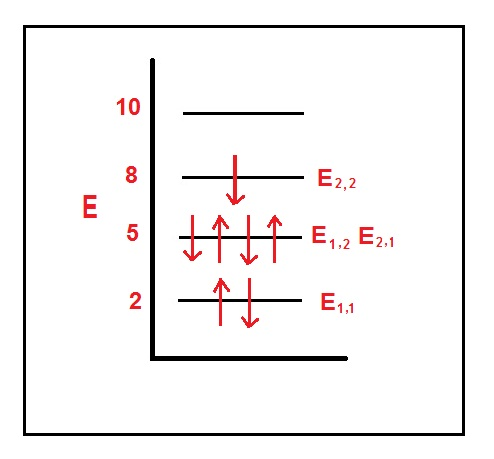
\includegraphics[width=5in]{../24/CH41/EX41.3/Example41_3a.jpg}
\caption{Sample Problem 3}
\end{figure}

\vspace*{10mm}
\curlable{Exa~41.4}
\begin{code}
\tcaption{Sample Problem 4}
\begin{verbatim}
Sample Problem 4
\end{verbatim}
\lstinputlisting{../24/CH41/EX41.4/Example41_4.sce}
\end{code}

\vspace*{10mm}
\vspace*{10mm}
\curlable{Exa~41.5}
\begin{code}
\tcaption{Sample Problem 5}
\begin{verbatim}
Sample Problem 5
\end{verbatim}
\lstinputlisting{../24/CH41/EX41.5/Example41_5.sce}
\end{code}

\vspace*{10mm}
\vspace*{10mm}
\curlable{Exa~41.6}
\begin{code}
\tcaption{Sample Problem 6}
\begin{verbatim}
Sample Problem 6
\end{verbatim}
\lstinputlisting{../24/CH41/EX41.6/Example41_6.sce}
\end{code}

\vspace*{10mm}
\chapter{Conduction of Electricity in Solids}

\vspace*{10mm}
\curlable{Exa~42.1}
\begin{code}
\tcaption{Sample Problem 1}
\begin{verbatim}
Sample Problem 1
\end{verbatim}
\lstinputlisting{../24/CH42/EX42.1/Example42_1.sce}
\end{code}

\vspace*{10mm}
\vspace*{10mm}
\curlable{Exa~42.2}
\begin{code}
\tcaption{Sample Problem 2}
\begin{verbatim}
Sample Problem 2
\end{verbatim}
\lstinputlisting{../24/CH42/EX42.2/Example42_2.sce}
\end{code}

\vspace*{10mm}
\vspace*{10mm}
\curlable{Exa~42.3}
\begin{code}
\tcaption{Sample Problem 3}
\begin{verbatim}
Sample Problem 3
\end{verbatim}
\lstinputlisting{../24/CH42/EX42.3/Example42_3.sce}
\end{code}

\vspace*{10mm}
\vspace*{10mm}
\curlable{Exa~42.4}
\begin{code}
\tcaption{Sample Problem 4}
\begin{verbatim}
Sample Problem 4
\end{verbatim}
\lstinputlisting{../24/CH42/EX42.4/Example42_4.sce}
\end{code}

\vspace*{10mm}
\vspace*{10mm}
\curlable{Exa~42.5}
\begin{code}
\tcaption{Sample Problem 5}
\begin{verbatim}
Sample Problem 5
\end{verbatim}
\lstinputlisting{../24/CH42/EX42.5/Example42_5.sce}
\end{code}

\vspace*{10mm}
\vspace*{10mm}
\curlable{Exa~42.6}
\begin{code}
\tcaption{Sample Problem 6}
\begin{verbatim}
Sample Problem 6
\end{verbatim}
\lstinputlisting{../24/CH42/EX42.6/Example42_6.sce}
\end{code}

\vspace*{10mm}
\vspace*{10mm}
\curlable{Exa~42.7}
\begin{code}
\tcaption{Sample Problem 7}
\begin{verbatim}
Sample Problem 7
\end{verbatim}
\lstinputlisting{../24/CH42/EX42.7/Example42_7.sce}
\end{code}

\vspace*{10mm}
\chapter{Nuclear Physics}

\vspace*{10mm}
\curlable{Exa~43.1}
\begin{code}
\tcaption{Sample Problem 1}
\begin{verbatim}
Sample Problem 1
\end{verbatim}
\lstinputlisting{../24/CH43/EX43.1/Example43_1.sce}
\end{code}

\vspace*{10mm}
\vspace*{10mm}
\curlable{Exa~43.2}
\begin{code}
\tcaption{Sample Problem 2}
\begin{verbatim}
Sample Problem 2
\end{verbatim}
\lstinputlisting{../24/CH43/EX43.2/Example43_2.sce}
\end{code}

\vspace*{10mm}
\vspace*{10mm}
\curlable{Exa~43.3}
\begin{code}
\tcaption{Sample Problem 3}
\begin{verbatim}
Sample Problem 3
\end{verbatim}
\lstinputlisting{../24/CH43/EX43.3/Example43_3.sce}
\end{code}

\vspace*{10mm}
\vspace*{10mm}
\curlable{Exa~43.4}
\begin{code}
\tcaption{Sample Problem 4}
\begin{verbatim}
Sample Problem 4
\end{verbatim}
\lstinputlisting{../24/CH43/EX43.4/Example43_4.sce}
\end{code}

\vspace*{10mm}
\vspace*{10mm}
\curlable{Exa~43.5}
\begin{code}
\tcaption{Sample Problem 5}
\begin{verbatim}
Sample Problem 5
\end{verbatim}
\lstinputlisting{../24/CH43/EX43.5/Example43_5.sce}
\end{code}

\vspace*{10mm}
\vspace*{10mm}
\curlable{Exa~43.6}
\begin{code}
\tcaption{Sample Problem 6}
\begin{verbatim}
Sample Problem 6
\end{verbatim}
\lstinputlisting{../24/CH43/EX43.6/Example43_6.sce}
\end{code}

\vspace*{10mm}
\vspace*{10mm}
\curlable{Exa~43.7}
\begin{code}
\tcaption{Sample Problem 7}
\begin{verbatim}
Sample Problem 7
\end{verbatim}
\lstinputlisting{../24/CH43/EX43.7/Example43_7.sce}
\end{code}

\vspace*{10mm}
\vspace*{10mm}
\curlable{Exa~43.8}
\begin{code}
\tcaption{Sample Problem 8}
\begin{verbatim}
Sample Problem 8
\end{verbatim}
\lstinputlisting{../24/CH43/EX43.8/Example43_8.sce}
\end{code}

\vspace*{10mm}
\vspace*{10mm}
\curlable{Exa~43.9}
\begin{code}
\tcaption{Sample Problem 9}
\begin{verbatim}
Sample Problem 9
\end{verbatim}
\lstinputlisting{../24/CH43/EX43.9/Example43_9.sce}
\end{code}

\vspace*{10mm}
\vspace*{10mm}
\curlable{Exa~43.10}
\begin{code}
\tcaption{Sample Problem 10}
\begin{verbatim}
Sample Problem 10
\end{verbatim}
\lstinputlisting{../24/CH43/EX43.10/Example43_10.sce}
\end{code}

\vspace*{10mm}
\chapter{Energy from the Nucleus}

\vspace*{10mm}
\curlable{Exa~44.1}
\begin{code}
\tcaption{Sample Problem 1}
\begin{verbatim}
Sample Problem 1
\end{verbatim}
\lstinputlisting{../24/CH44/EX44.1/Example44_1.sce}
\end{code}

\vspace*{10mm}
\vspace*{10mm}
\curlable{Exa~44.2}
\begin{code}
\tcaption{Sample Problem 2}
\begin{verbatim}
Sample Problem 2
\end{verbatim}
\lstinputlisting{../24/CH44/EX44.2/Example44_2.sce}
\end{code}

\vspace*{10mm}
\vspace*{10mm}
\curlable{Exa~44.3}
\begin{code}
\tcaption{Sample Problem 3}
\begin{verbatim}
Sample Problem 3
\end{verbatim}
\lstinputlisting{../24/CH44/EX44.3/Example44_3.sce}
\end{code}

\vspace*{10mm}
\vspace*{10mm}
\curlable{Exa~44.4}
\begin{code}
\tcaption{Sample Problem 4}
\begin{verbatim}
Sample Problem 4
\end{verbatim}
\lstinputlisting{../24/CH44/EX44.4/Example44_4.sce}
\end{code}

\vspace*{10mm}
\vspace*{10mm}
\curlable{Exa~44.5}
\begin{code}
\tcaption{Sample Problem 5}
\begin{verbatim}
Sample Problem 5
\end{verbatim}
\lstinputlisting{../24/CH44/EX44.5/Example44_5.sce}
\end{code}

\vspace*{10mm}
\vspace*{10mm}
\curlable{Exa~44.6}
\begin{code}
\tcaption{Sample Problem 6}
\begin{verbatim}
Sample Problem 6
\end{verbatim}
\lstinputlisting{../24/CH44/EX44.6/Example44_6.sce}
\end{code}

\vspace*{10mm}
\chapter{Quarks Leptons and the Big Bang}

\vspace*{10mm}
\curlable{Exa~45.1}
\begin{code}
\tcaption{Sample Problem 1}
\begin{verbatim}
Sample Problem 1
\end{verbatim}
\lstinputlisting{../24/CH45/EX45.1/Example45_1.sce}
\end{code}

\vspace*{10mm}
\vspace*{10mm}
\curlable{Exa~45.2}
\begin{code}
\tcaption{Sample Problem 3}
\begin{verbatim}
Sample Problem 3
\end{verbatim}
\lstinputlisting{../24/CH45/EX45.2/Example45_2.sce}
\end{code}

\vspace*{10mm}
\vspace*{10mm}
\curlable{Exa~45.3}
\begin{code}
\tcaption{Sample Problem 3}
\begin{verbatim}
Sample Problem 3
\end{verbatim}
\lstinputlisting{../24/CH45/EX45.3/Example45_3.sce}
\end{code}

\vspace*{10mm}
\vspace*{10mm}
\curlable{Exa~45.6}
\begin{code}
\tcaption{Sample Problem 6}
\begin{verbatim}
Sample Problem 6
\end{verbatim}
\lstinputlisting{../24/CH45/EX45.6/Example45_6.sce}
\end{code}

\vspace*{10mm}
\vspace*{10mm}
\curlable{Exa~45.7}
\begin{code}
\tcaption{Sample Problem 7}
\begin{verbatim}
Sample Problem 7
\end{verbatim}
\lstinputlisting{../24/CH45/EX45.7/Example45_7.sce}
\end{code}

\vspace*{10mm}
\chapter*{Appendix}

\curlable{AP~1}
\begin{code}
\label{AP:285}
\tcaption {Modern Physics}{Modern Physics}
\lstinputlisting{../24/DEPENDENCIES/quantum.sci}
\end{code}

\curlable{AP~2}
\begin{code}
\label{AP:272}
\tcaption {degree_rad}{degree_rad}
\lstinputlisting{../24/DEPENDENCIES/degree_rad.sci}
\end{code}

\curlable{AP~3}
\begin{code}
\label{AP:273}
\tcaption {gravitation}{gravitation}
\lstinputlisting{../24/DEPENDENCIES/Gravitation.sci}
\end{code}

\curlable{AP~4}
\begin{code}
\label{AP:284}
\tcaption {electrostatic}{electrostatic}
\lstinputlisting{../24/DEPENDENCIES/electrostatics.sci}
\end{code}

\curlable{AP~5}
\begin{code}
\label{AP:283}
\tcaption {Example 17-1}{Example 17-1}
\lstinputlisting{../24/DEPENDENCIES/Example17_1.sce}
\end{code}

\curlable{AP~6}
\begin{code}
\label{AP:282}
\tcaption {Bernauli's Equation}{Bernauli's Equation}
\lstinputlisting{../24/DEPENDENCIES/Bernauli.sci}
\end{code}

\curlable{AP~7}
\begin{code}
\label{AP:277}
\tcaption {Cross Product}{Cross Product}
\lstinputlisting{../24/DEPENDENCIES/cross_product.sci}
\end{code}

\curlable{AP~8}
\begin{code}
\label{AP:281}
\tcaption {Example 11-7}{Example 11-7}
\lstinputlisting{../24/DEPENDENCIES/Example11_7.sce}
\end{code}

\curlable{AP~9}
\begin{code}
\label{AP:280}
\tcaption {collision}{collision}
\lstinputlisting{../24/DEPENDENCIES/collision.sci}
\end{code}

\curlable{AP~10}
\begin{code}
\label{AP:279}
\tcaption {Example 4-3}{Example 4-3}
\lstinputlisting{../24/DEPENDENCIES/Example4_3.sce}
\end{code}

\curlable{AP~11}
\begin{code}
\label{AP:278}
\tcaption {Example 4-2a}{Example 4-2a}
\lstinputlisting{../24/DEPENDENCIES/Example4_2a.sce}
\end{code}

\curlable{AP~12}
\begin{code}
\label{AP:276}
\tcaption {Example 2-1b}{Example 2-1b}
\lstinputlisting{../24/DEPENDENCIES/Example2_1b.sce}
\end{code}

\curlable{AP~13}
\begin{code}
\label{AP:275}
\tcaption {Example 2-1a}{Example 2-1a}
\lstinputlisting{../24/DEPENDENCIES/Example2_1a.sce}
\end{code}

\end{document}
